\documentclass[11pt,a4paper,twoside,openright]{report}

\usepackage{amsmath}
\usepackage{amssymb}
\usepackage{amsthm}
\usepackage[titletoc]{appendix}
\usepackage{bm}
\usepackage{cite}
\usepackage{graphicx}
\usepackage{hyperref}
\usepackage{setspace}
\usepackage{subfigure}

% No paragraph indentation, newline between paragraphs
\usepackage[parfill]{parskip}

\graphicspath{ {images/} }

\author{Catherine Vlasov}
\title{Empirical Validation of the Square Root Law of Steganography}

% To make the text centered when report is bound
\addtolength{\oddsidemargin}{10mm}
\addtolength{\evensidemargin}{-10mm}

\begin{document}

\makeatletter
  \begin{titlepage}
    \vspace*{\fill}
      \begin{center}
        {\setstretch{1.5} \huge \bfseries \@title \par}
        \vspace{20ex}
        \includegraphics[width=30mm]{oxlogo.png}
        \\[10ex]
        {\LARGE \@author}
        \\[3ex]
        {\Large University College}
        \\[1ex]
        {\Large University of Oxford}
        \\[8ex]
        {\Large Honour School of Computer Science}
        \\[1ex]
        {\Large \emph{Computer Science Project (Part C)}}
        \\[10ex]
        {\LARGE May 2019}
      \end{center}
    \vspace*{\fill}
  \end{titlepage}
\makeatother


\shipout\null


%-----------------------
\begin{abstract}

Abstract.

\end{abstract}


\shipout\null
\pagenumbering{roman}

%-----------------------
\tableofcontents

\cleardoublepage
\pagenumbering{arabic}
\newpage

%-----------------------
\chapter{Introduction}

On July 5, 2018, Xiaoqing Zheng emailed himself an image of a sunset \cite{info-sec-ge}. On April 23, 2019, he was arraigned by U.S. authorities \cite{washington-post-ge}. Why? The answer was hidden in plain sight.

Public channels can be used to share information in plaintext (such as public keys) or private information using encryption (like personal messages). All such messages are visible to eavesdroppers, who can tell which people are communicating, how often they do so, and how much information they are sharing. However, a third use case is gaining popularity: hiding one message inside another to make the hidden message invisible to eavesdroppers. This is called steganography -- the art of hiding information.

Zheng is part of a growing trend of using steganography in cyber attacks. The sunset image  he emailed to his personal address while working at General Electric (GE) looked innocent to the naked eye -- and to GE's intrusion detection system -- but it concealed 40 Excel and MATLAB files \cite{info-sec-ge}. This is one of many examples of steganography being used outside an academic context.

Banner advertisements \cite{forbes-banner-ads}, memes \cite{trend-micro-memes}, and even the $16\times16$ pixel ``favicons" shown beside website names in browser tabs \cite{trend-micro-steganography} have been used for steganography -- in many cases to spread malware. It is therefore important for the security community to understand how steganography works and, crucially, how best to detect it. Detecting whether or not an image has a hidden payload is a binary classification task, but its difficulty varies greatly with the length of the payload. A well-trained classifier is likely to identify images with large hidden payloads with high accuracy, but its accuracy is likely to drop significantly as the payload size decreases.

This project studies precisely this behaviour. In particular, the aim is to empirically validate the ``square root law", which quantifies\footnote{Is this the right/best word choice?} the relationship between payload size and classifier accuracy. Intuitively (and informally), the law states that detectability remains constant if the payload size is proportional to the \textit{square root} of the number of pixels in an image, all other things being equal. The law was conjectured in 2006 \cite{batch-first-srl} and then empirically validated in 2008 using state-of-the-art (at the time) embedding and detection algorithms \cite{2008-paper}. The results in \cite{2008-paper} are now -- more than a decade later -- out of date given how far the field has progressed and this project provides fresh results, using the current best available tools and techniques. We will find that the square root law still appears to hold by running computation-intensive experiments on two large sets of images.

As discussed in \cite{2008-paper}, this result is significant because it puts into question what unit of measurement is most meaningful when describing the capacity of an image (the amount of information that can be embedded inside it). Instead of ``bits per pixel", should it be ``bits per square root pixel"? In addition, the square root law has practical implications for users of steganographic algorithms. When deciding how much payload to embed, should they consider the maximum number of bits that can ``physically" fit in an image or some other capacity measurement?

In addition to mirroring the experiments in \cite{2008-paper}, we explore an idea mentioned in the paper's conclusion: steganographic capacity might be more precisely modelled as being proportional to $\sqrt{N} \cdot \log{N}$ (where $N$ is the number of pixels in an image). This also yields promising results.


\section{Outline}

In Chapter 2, I will provide background on the field of steganography, including necessary terminology as well as  progress made in embedding and detection techniques since 2008, when \cite{2008-paper} was published. This context will lead into technical descriptions of the algorithms I chose. Then I will introduce a precise mathematical formulation of the square root law and give an overview of important caveats related to its practical application. Finally, I will discuss the project's goals.

Chapter 3 covers the design, implementation, and running of the experiments. I begin by outlining the experiment requirements and then explain each component of my experiment pipeline. The chapter provides sufficient detail to replicate my results, given access to the image sets and relevant code.

Then, Chapter 4 presents, describes, and analyzes the experiment results. The result graphs mimic the style used in \cite{2008-paper} and align nicely with the expected behaviour.

Finally, Chapter 5 summarizes my findings, discusses interesting and potentially fruitful areas of further research, revisits the project goals, and discusses how they were achieved.


%-----------------------
\chapter{Background}

To see why this project was undertaken, we need to understand its context: the current state of steganography as well as its state ten years ago.

I will start by introducing key steganography terminology and concepts as well as how JPEG compression works. Then I will discuss some of today's best-known embedding and detection algorithms and compare them to the best techniques at the time \cite{2008-paper} was written. Finally, I will give a precise formulation of the square root law and lay out this project's goals.


\section{Steganography}

The word ``steganography" comes from the combination of the Greek words ``steganos" (meaning ``covered") and ``graphia" (meaning ``writing") \cite{textbook}. The first known use of steganography \cite[\S 1.1]{textbook} is documented in Herodotus' influential \textit{The Histories} \cite{herodotus}, written in 440 BC. He describes how a secret message is tattooed on the scalp of a slave, the slave's hair grows back to conceal the message, and he is sent to another city. Upon arrival, his head is shaved to reveal the message to the intended recipient.

This story can be boiled down to an instance of Simmons' famous prisoner's problem, which was first proposed in 1983 \cite{prisoners-problem}. Two Prisoners are locked in separated cells but are allowed to communicate, subject to the monitoring of their messages by a Warden. Using steganography, they can secretly exchange messages that the Warden cannot see and therefore cannot read. However, if the Warden detects that they are communicating secretly, their steganographic system is broken.

So far, we have informally been referring to two concepts: embedding and detection. In the context of the prisoner's problem, the Prisoners are like Embedders and the Warden is like a Detector. These concepts are in fact part of two separate, through closely related, fields: \textbf{steganography} and \textbf{steganalysis}. The former is the study of \textit{hiding} information whereas the latter is the study of \textit{detecting} hidden information. An object that has not been modified is referred to as a \textbf{cover object} and an object with an embedded message is called a \textbf{stego object}. The input to an \textbf{embedding algorithm} is a cover object, a secret message (called the \textbf{payload}), and a secret key shared by the sender and receiver and the output is a stego object. Notice, however, that an embedding algorithm without a corresponding means for the recipient of a stego object to read the secret message is useless. Thus, every embedding algorithm has a matching \textbf{extraction algorithm} whose input is a stego object and a secret key and output is the hidden payload. The embedding and extraction algorithms, together with the sources of cover objects (for instance a camera or microphone), secret keys, and payloads as well as the communication channel (like an email service), make up a \textbf{stegosystem} \cite{ker-notes}.

In a modern context, the ``objects" used for steganography are commonly digital media such as images, MP3 files, and videos. In this project we will study JPEG steganography, which makes use of properties of the JPEG compression algorithm (described in Section \ref{sec:jpeg-compression}) to hide information.

The aim of steganography is to make it impossible for an eavesdropper to decide whether or not an object contains a hidden payload. A stegosystem that fulfills this goal is called \textbf{secure}. In addition, an aim of steganography researchers is to design embedding and extraction algorithms that maximize a stegosystem's \textbf{capacity}: the maximum payload size. However, these two aims are in direct competition. An unsatisfying (and useless) way of fulfilling the first aim is to always choose a payload of size zero -- like this, the cover and stego objects are identical and therefore an eavesdropper cannot, by definition, distinguish between them. However, this does not seem to ``maximize" the payload size in any sense of the word. On the other hand, defining capacity as the maximum number of bits $N$ that ``physically" fit in a cover object (say the total number of bits used to store a JPEG file) and attempting to hide an $N$-bit payload is very likely to make the stego object look like a garbled sequence of bits that no longer even has the correct format to be parsed as a JPEG file. Therefore, a detector will likely identify all such objects with near perfect accuracy.

As we can see, it is difficult to define the concept of capacity precisely. Despite its lack of a formal definition, capacity is often measured as an \textbf{embedding rate}; that is, payload size relative to cover size, such as bits per cover pixel. This project does not attempt to define capacity, but rather shine a light on what its most appropriate unit of measurement might be, in the context of JPEG steganography. 


\section{JPEG Compression} \label{sec:jpeg-compression}

I will now briefly describe how JPEG compression works. A complete, detailed description can be found in \cite{jpeg-standard}.

What makes JPEG compression space-efficient is \textbf{quantization}: for any $x \in \mathbb{R}$ and constant \textbf{quantization factor} $q$, we have $x \approx q [x/q]$ (where $[ \cdot ]$ is the nearest integer function). Instead of storing $x$, we can store $[x/q]$, which is small for large enough $q$.

An RGB colour bitmap image is a raw image where each pixel is stored as three bytes representing the red, green, and blue colour intensities, respectively. JPEG compression of such an image involves five steps.

\paragraph{Step 1: Colour space transformation} Each pixel is separated into one luminance (brightness) component and two chrominance (colour) components via a linear transformation. The human visual system is more sensitive to changes in brightness than in colour \cite{textbook}, so JPEG reduces the resolution of the chrominance components for storage efficiency and only uses the luminance component for embedding. For this reason, the descriptions of the remaining steps are described only for luminance -- the chrominance components undergo a similar process.

\paragraph{Step 2: Division into blocks} The $W \times H$ image is split into $\lceil W/8 \rceil \times \lceil H/8 \rceil$ blocks of $8 \times 8$ luminance values. Zero padding is used if either dimension is not a multiple of 8.

\paragraph{Step 3: Discrete cosine transform (DCT)} This is the heart of the algorithm and is similar to the discrete Fourier transform. The DCT transforms the image into another domain that is easier to compress due to its sparsity, at the expense of being lossy. Specifically, the \textbf{spatial domain} is transformed to the \textbf{frequency domain}\footnote{Do I need to explain these further?}. Each $8 \times 8$ block $\bm{B}$ of pixels undergoes the DCT to produce an $8 \times 8$ block $\bm{C}$ of frequencies (referred to as \textbf{coefficients}).

It is easiest to understand the transformation by considering its inverse. The goal is to choose coefficients $\bm{C}[u,v]$ for $u,v = 0,...,7$ such that:
\begin{equation*}
    \bm{B} = \sum_{u=0}^7 \sum_{v=0}^7 \bm{C}[u,v] \bm{A_{u,v}}
\end{equation*}

for \textbf{DCT modes} $\bm{(u,v)}$. The transformation is effectively an orthonormal change of basis where the blocks $\bm{A_{u,v}}$ make up the basis and the coefficients $\bm{C}$ define the linear combination of these basis blocks. Coefficient $\bm{C}[0,0]$ is called the \textbf{DC coefficient} and the remaining coefficients are called \textbf{AC coefficients}.

The $\bm{A_{u,v}}$ are defined as follows for $i,j = 0,...,7$ and where $c_0=1$ and $c_i=\sqrt{2}$ for all $i > 0$:
\begin{equation*}
    \bm{A_{u,v}}[i,j] = \frac{c_u c_v}{8} \cos{\Bigg(\frac{\pi}{8}\Big(i + \frac{1}{2}\Big)u\Bigg)} \cos{\Bigg(\frac{\pi}{8}\Big(j + \frac{1}{2}\Big)v\Bigg)}
\end{equation*}

\begin{figure}[htbp] 
	\begin{center}
		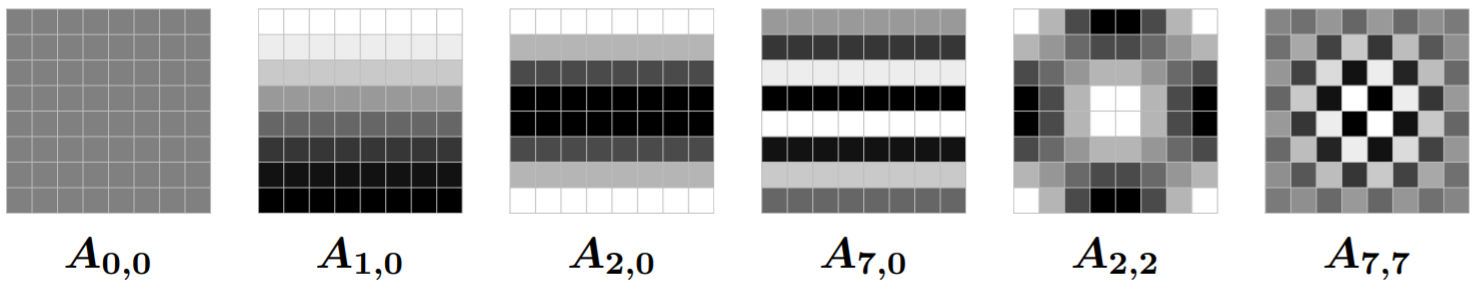
\includegraphics[width=0.75\linewidth]{dct_basis_examples.png}
		\caption{A few examples of DCT basis blocks \cite{ker-notes}.}
		\label{fig:dct-basis-examples}
	\end{center}
\end{figure}

Figure \ref{fig:dct-basis-examples} shows a few examples of these blocks. The result of this step is that the high- and low-frequency parts of each luminance block $\bm{B}$\footnote{Is this correct?} are separated.

\paragraph{Step 4: Quantization} Most of the lost information is due to this step because quantization (dividing by a number then rounding to the nearest integer) is a many-to-one operation. Within each block $\bm{C}$, each coefficient is quantized separately, with larger coefficients getting larger quantization factors than smaller coefficients. A matrix of quantization factors $\bm{Q}_{qf}$ can be determined according to the \textbf{quality factor} $qf$ (an integer\footnote{?} between 1 and 100, inclusive) chosen for the compression. Thus, instead of storing $\bm{C}[i,j]$, we store\footnote{Do I need to mention again that [.] is the nearest integer function?}:
\begin{equation*}
	\Bigg[ \frac{\bm{C}[i,j]}{\bm{Q}_{qf}[i,j]} \Bigg]
\end{equation*}

Low quality factors have result in larger quantization factors, which cause more coefficients to be quantized to zero. Therefore the compression is more efficient, at the expense of more information being lost.

\paragraph{Step 5: Encoding} This step is not relevant for this project and a full description can be found in \cite{jpeg-standard}. It involves encoding the matrix of quantization factors as well as the quantized coefficients (stored based on a zig-zag ordering in order to increases the changes of runs of zeros for better compressibilitiy). These make it possible for the quantization to be approximately reversed during decompression by multiplying each quantized coefficient by the corresponding element of the quantization factor matrix and performing the inverse discrete cosine transform.


\section{JPEG Steganography} \label{sec:jpeg-steganography}

Now that we understand how JPEG compression works, we can explore how to use JPEG images as a medium for steganography.

One of the simplest embedding algorithms, called \textbf{least significant bit replacement (LSBR)} uses the least significant bit (LSB) of each pixel to carry one bit of the payload\footnote{This assumes we use a grayscale image where each pixel is represented as a single byte. In the case of a colour RGB image, we can use each RGB byte to store one bit of payload.}. This works for raw, uncompressed images (though it is highly detectable \cite{ker-notes}), but not for JPEGs due to the information loss during the quantization step. However, we can still use this idea, except \textit{after} information is lost.

Instead of overwriting the LSB of each pixel, we can modify the LSB of each quantized (luminance) DCT coefficient\footnote{Since the luminance channel is almost always the one used for embedding, I will no longer specifically mention this when discussing the use of coefficients for embedding. I will also omit the term ``quantized'' and assume this to be implied, in the context of embedding.} by adding or subtracting one. This is the central idea behind most JPEG embedding algorithms.

Modifying coefficients that are equal to zero tends to have a visually perceptive effect on the decompressed image, particularly in smooth areas (like the sky). Thus, changing such coefficients is typically avoided and so the capacity of JPEG images is typically measured in terms of bits per non-zero DCT coefficient. Changes to the (0,0) DCT mode -- which is featured in Figure \ref{fig:dct-basis-examples} -- are also highly detectable because they cause blocks of $8\times8$ pixels to appear brighter or dimmer. This is therefore also generally avoided \cite{ker-notes}.


\subsection{Progress in the Last Decade} \label{sec:embed-progress}

One of the best-known JPEG embedding methods at the time \cite{2008-paper} was written is called \textbf{F5}. Each bit of the payload is embedded in a non-zero coefficient by modifying the coefficient's LSB -- if this results in the coefficient becoming equal to zero, then the same bit is embedded again in the next non-zero coefficient \cite{f5}. Two consequences of this repeated embedding is that the capacity of images is relatively low and coefficients get pulled towards zero. The latter effect is referred to as ``shrinkage" and it means that the number of zero-valued coefficients increases, therefore increasing detectability. In \textbf{no shrinkage F5} (referred to as \textbf{ns-F5}), the effect of pulling coefficients towards zero is eliminated using wet paper codes \cite{no-shrinkage-f5} (a topic beyond the scope of this report).

F5 was the leading JPEG embedding algorithm over a decade ago \cite{ker-notes} and nsF5 was the algorithm chosen to represent ``state-of-the-art'' embedding in \cite{2008-paper}. However, a lot of progress in the development embedding methods has been made since then. In particular, an idea called \textbf{adaptive embedding} has since been studied in great depth: it aims to identify embedding changes (such as modifications to the LSB of a coefficient) in parts of an image that are the least detectable \cite{ker-notes}. This led to the development of new embedding tools like J-UNIWARD (described in Section \ref{sec:juniward}), the one used in this project.

Currently, one of the most common approaches to designing embedding algorithms is finding a way to embed a payload while minimizing a \textbf{distortion} function \cite{costs-and-capacity}. A parallel to this is constructing a machine learning model that makes predictions while minimizing a cost function like least squares. A formal definition of this task is discussed in Section \ref{sec:distortion-function-min}. In fact, an additive approximation of the distortion function is used to simplify the embedding algorithm and assign a cost for changing each DCT coefficient (in the case of JPEGs). In addition, Syndrome-Trellis Codes (STCs) are a standard tool used to implement the embedding -- more details about them can be found in \cite{stc-paper}.


\subsection{Distortion Function Minimization} \label{sec:distortion-function-min}

We will now formalize the task of embedding while minimizing a distortion function. This is partially based on the formulation in \cite{stc-paper}, which I have adapted to describe embedding in JPEGs. I will skip over some logistical details in the interest of conciseness, but a full account is in \cite{stc-paper}.

Let $\bm{x} = (x_1,...,x_n) \in \mathcal{X} = \mathcal{I}^n$ be a cover image, expressed as a sequence of $n$ quantized DCT coefficients. We will treat $\bm{x}$ as being \textit{constant} and so we will not explicitly express dependence on it.

Similarly, let $\bm{y} = (y_1,...,y_n) \in \mathcal{Y} = \mathcal{I}_1 \times ... \times \mathcal{I}_n$ be a stego image. Each $\mathcal{I}_i$ satisfies $\mathcal{I}_i \subset \mathcal{I}$ and $x_i \in \mathcal{I}_i$ (representing the case where a coefficient is not modified). We say embedding is \textbf{binary} if $| \mathcal{I}_i | = 2$ for all $i$ or \textbf{ternary} if $| \mathcal{I}_i | = 3$ for all $i$. Changing coefficients by $\pm 1$, for instance, has $\mathcal{I}_i = \{ x_i-1, x_i, x_i+1 \}$. In this project, however, we are interested in binary embedding algorithms because the algorithms tested in \cite{2008-paper} were binary.

Let $\mathcal{D} : \mathcal{X} \to \mathbb{R}$ be a distortion function. Since $\bm{x}$ is constant, we write $\mathcal{D}(\bm{y})$ instead of $\mathcal{D}(\bm{x},\bm{y})$, which expresses the total cost of modifying the coefficients that differ in $\bm{x}$ and $\bm{y}$. We are interested in additive distortion functions, meaning that they can be written as:
\begin{equation*}
	\mathcal{D}(\bm{x},\bm{y}) = \sum_{i=1}^n \rho_i(\bm{x},y_i)
\end{equation*}
where $\rho_i$ is a function that gives a bounded cost for replacing cover pixel $x_i$ with $y_i$. If $y_i \notin \mathcal{I}_i$, we say $\rho_i(\bm{x},y_i) = \infty$. Notice that $\rho_i$ depends on the entire cover image, meaning that it can make use of relationships between coefficients, but it does \textit{not} depend on any other $\rho_j$ (where $i \neq j$), meaning that embedding changes are independent.

Here, we will diverge slightly from the formulation given in \cite{stc-paper} and express everything in terms of individual coefficients rather than the cover as a whole. This is a bit easier to understand.

We assume that our embedding algorithm computes probabilities $\pi_1,...,\pi_n$ such that $\pi_i$ is the probability that coefficient $x_i$ is modified. In the context of binary embedding, this means that with probability $1-\pi_i$ coefficient $x_i$ is untouched and with probability $\pi_i$ coefficient $x_i$ is either incremented or decremented by 1 (this decision is made uniformly at random). This is in contrast with ternary embedding where there are three probabilities: one for making no change, one for adding 1, one for subtracting 1.

We now introduce the binary entropy function from information theory:
\begin{equation*}
	h(x) = -x \cdot \log_2 x - (1-x) \cdot \log_2{(1-x)}
\end{equation*}

Finally, let $c_i = \rho_i(\bm{x},y_i)$. 

Tying everything together, we can express the problem of embedding while minimizing a distortion function as two optimization problems, which are actually dual to each other:
\begin{enumerate}

	\item \textbf{Payload-limited sender (PLS)}: Embed a payload of a \textit{fixed} length of $m$ bits while minimizing the average distortion:
		\begin{equation*}
			\begin{aligned}
			& \underset{\pi_1,...,\pi_n}{\text{Minimize}}
			& & \sum_{i=1}^{n} c_i \pi_i \\
			& \text{subject to}
			& & \sum_{i=1}^{n} h(\pi_i) \geq m
			\end{aligned}
		\end{equation*}

	\item \textbf{Distortion-limited sender (DLS)}: Given a fixed average distortion $C_{\epsilon}$, embed a payload of maximum length:
		\begin{equation*}
			\begin{aligned}
			& \underset{\pi_1,...,\pi_n}{\text{Maximize}}
			& & \sum_{i=1}^{n} h(\pi_i) \\
			& \text{subject to}
			& & \sum_{i=1}^{n} c_i \pi_i \geq C_{\epsilon}
			\end{aligned}
		\end{equation*}

\end{enumerate}

From a practical perspective, PLS is a more natural formulation because someone wanting to send a message tends to have a particular message in mind. Since PLS and DLS are dual to each other, the optimal solution for one is also optimal for the other and this can be computed to be (full derivation in \cite{stc-paper}, for some fixed $\lambda$:
	\begin{equation} \label{eq:prob-i}
		\pi_i = \frac{\exp{(-\lambda c_i)}}{\exp{(-\lambda c_i)} + \exp{(-\lambda c_i^{\ast})}} = \frac{1}{\exp{(-\lambda c_i)} + 1}
	\end{equation}
where $c_i^{\ast}$ is the cost of \textit{not} changing coefficient $x_i$. In \eqref{eq:prob-i} we assume $c_i^{\ast} = 0$, but a non-zero cost is possible in a scenario where making a change is actually beneficial, but we consider this to be beyond the scope of this project.

This optimal solution occurs when $\sum_{i=1}^{n} h(\pi_i) = m$ because $\sum_{i=1}^{n} h(\pi_i)$ is a monotonically increasing function. We can therefore pick a value of $\lambda$ such that the equality holds for any value of $m$ we want and compute the probabilities $\pi_i$ with \eqref{eq:prob-i}.

The key take-away here is that we can \textit{simulate} the embedding of an $m$-bit payload by changing each pixel with probability $\pi_i$. This is precisely what J-UNIWARD, the embedding algorithm I used in this project, does. It is described in more detail in Section \ref{sec:juniward}.


\subsection{J-UNIWARD} \label{sec:juniward}

UNIWARD (``universal wavelet relative distortion") \cite{uniward-paper} is a distortion function that forms the basis of several embedding methods. The term ``universal" refers to the fact that UNIWARD can operate on any domain, such as the \textbf{spatial} domain (where the payload is hidden in the pixels) and the \textbf{JPEG domain} (where the payload is hidden in the DCT coefficients - also called the \textbf{DCT domain} or \textbf{transform domain}).

The UNIWARD distortion function is the sum of relative changes to wavelet coefficients with respect to the cover image . The wavelet coefficients come from three directional wavelet filter banks, which effectively measure the horizontal, vertical, and diagonal smoothness of an image. A more technical description of filter banks and wavelets is beyond the scope of this project and can be found in \cite{uniward-paper}. As is standard practice, an additive approximation of the function is used for the embedding.

J-UNIWARD is one of the embedding algorithms based on the UNIWARD distortion function and it operates in the JPEG domain. It has been shown \cite{uniward-paper} to significantly outperform nsF5 and another former state-of-the-art algorithm called UED (uniform embedding distortion) and an implementation is freely available online for research purposes \cite{binghamton-embedding}, thus making it a good choice for this project.


\section{JPEG Steganalysis}

Steganalysis is a supervised binary classification problem. Given a set of training data (consisting of a feature vector and a ``cover'' or ``stego'' label for each of a large number of images), a \textbf{detector} learns how to distinguish cover images from stego images, represented in the feature space. To achieve the best results, features used in steganalysis should be sensitive to changes caused by embedding while being indifferent to the content of images. The majority of steganalysis methods are based on machine learning, but the types of models that perform best have varied over the years.


\subsection{Progress in the Last Decade} \label{sec:steganalysis-progress}

Advances in steganalysis over the last decade were mainly due to the development of the field of machine learning and therefore the development of richer and more meaningful feature sets.

A decade ago, features derived from DCT coefficients enabled classifiers to achieve the best performance in JPEG steganalysis. This is because features computed directly from the embedding domain (like RGB values for raw colour images and DCT coefficients for JPEG images) were considered to be the most sensitive to changes caused by embedding \cite{blind-steganalysis}.

However, feature spaces tended to be quite small: the features used in \cite{2008-paper} had only 274 dimensions. These so-called ``merged'' features combined:
\begin{enumerate}
  \item DCT features -- such as histograms of DCT coefficient values, histograms of coefficients of specific DCT modes, and dependencies between coefficients in different blocks
  \item Markov features -- these are derived from a Markov process that models differences between the absolute values of neighboring DCT coefficients
\end{enumerate}
They were used to build a blind\footnote{A classifier with no prior knowledge of what embedding algorithm is likely to be used is called ``blind''. For this reason, the features it takes as input must be generic as opposed to being designed to capture specific properties of images that are known to be modified by a certain embedding algorithm.} multi-class classifier for (single-compressed\footnote{This means that the JPEG image was produced by compressing a raw image that was never compressed before. Images that have been compressed, decompressed, then compressed again (for instance) have different properties than single-compressed images due to the loss of information and therefore cannot be treated as equivalent to single-compressed images.}) JPEG images based on soft-margin support vector machines (SVMs) with Gaussian kernels \cite{2008-features}. The classifier used $\binom{7}{2}=21$ binary classifiers and the ``max wins'' method to classify images into one of seven classes: cover image or stego image produced by one of six embedding algorithms. This technique was considered state-of-the-art in 2008 and \cite{2008-paper} used the binary classifier trained to distinguish between cover images and images produced by F5 (discussed in \ref{sec:embed-progress})\footnote{Is this correct? I can't think of a reason you would have used the multi-classifier.}.

Today, a typical approach to steganalysis consists of defining an image model and a machine learning model trained to differentiate between cover and stego images (represented in the model) \cite{jrm-paper}. Image models continue to be based on the embedding domain, but tend to be much more complex than a decado ago. In the context of JPEG steganalysis, they capture properties of individual DCT coefficients (such as frequencies of coefficient values) as well as relationships between coefficients (like how often two values occur beside each other)\footnote{Rereading what I've written in this section, this sounds very similar to what was being done in 2008. Are there any more significant differences?}. This results in much richer -- and therefore larger -- feature sets that help classifiers achieve better results. The JPEG Rich Model (JRM) is one such model, which I used in this project and I describe in Section \ref{sec:jrm}.

In 2012, a well-known machine learning tool was put to use in steganalysis as a simpler and more scalable alternative to SVMs. Ensemble classifiers, implemented as random forests, came to light as a new tool with promising results -- they produced a better detection accuracy by combining the results of multiple individual classifiers \cite{ensemble-classifier}. However, only a few years later, it was shown that a properly regularized (and trained) linear classifier could perform just as well as an ensemble classifier, with a much lower computational complexity \cite{classifier-paper}. For this reason, I chose to use one such linear classifier for detection in my experiments, as discussed in Section \ref{sec:classifier-background}.


\subsection{JRM} \label{sec:jrm}

The Cartesian-calibrated JPEG Rich Model (CC-JRM) is a current state-of-the-art image model that produces a $22\,510$-dimensional feature space, irrespective of image size. The term ``rich'' refers to the model's complexity: it consists of a large number of submodels that are combined to produce the features. CC-JRM uses some interesting ideas, such as using the differences between the absolutes values of coefficients, and more details can be found in the original paper \cite{jrm-paper}.


\subsection{Low-Complexity Linear Classifier} \label{sec:classifier-background}

An implementation of a low-complexity linear classifier is available online \cite{binghamton-classifier} and I used it for my experiments. It takes a set of pairs of cover image features and corresponding stego image features as input and splits them 50/50 into a training set and a testing set, keeping cover-stego pairs together. Then, it selects a regularization parameter with 5-fold cross-validation on the training set and uses it to regularize the classifier. Finally, the classifier is run on the testing set and the probability of error is output.


\section{Square Root Law}

\subsection{Batch Steganographic Capacity} \label{sec:batch-capacity}

The so-called ``square root law'' (SRL) was first conjectured in 2006 in \cite{2006-batch-conjecture} in the context of \textbf{batch steganography}, where a payload is spread over a collection of objects. A year later, it was formalized and proven \cite{2007-batch-proof}. Finally, the law was empirically validated in 2008 both in the spatial domain (on raw images) and in the JPEG domain \cite{2008-paper}.

Theorem \ref{thm:square-root-law-batch} states the formalized SRL from \cite{2007-batch-proof}, exactly as paraphrased in \cite{2008-paper}:

\newtheorem{square-root-law}{Theorem}
\begin{square-root-law}[Batch Steganographic Capacity] \label{thm:square-root-law-batch}
If a steganographer embeds a total payload of M bits into N uniform cover objects, then:
\begin{enumerate}
	\item If $M/\sqrt{N} \to \infty$ as $N \to \infty$ then there is a pooled detector which, for sufficiently large $N$, comes arbitrarily close to perfect detection.
	\item If $M/\sqrt{N} \to 0$ as $N \to 0$ then, by spreading the payload equally between $N$ covers, the performance of any pooled detector must become arbitrarily close to random for sufficiently large $N$.
\end{enumerate}
\end{square-root-law}

A \textbf{pooled detector} is one that performs steganalysis on each of a sequence of $N$ objects \textit{separately} and then uses the results to decide whether the entire batch of objects contains a payload.

Although not directly relevant to this project, it is interesting to briefly mention two other versions of the SRL. In particular, the law has been shown to hold if the cover source can be modelled as a stationary Markov chain \cite{srl-markov-covers} or as a Markov Random Field (including inhomogeneous Markov chains and Ising models) \cite{srl-markov-random-fields}. Further details are beyond the scope of this report, but these results are significant because they prove that the law holds under more realistic assumptions about the cover source. Theorem \ref{thm:square-root-law-batch}, on the other hand assumes that the covers are uniform. This, and other assumptions are discussed in Section \ref{sec:srl-caveats}.


\subsection{Relation to Capacity of Individual Cover Objects}

How does Theorem \ref{thm:square-root-law-batch} -- a result about the steganographic capacity of \textit{batches} of object -- apply to the capacity of \textit{individual} cover objects? We can answer this by giving another interpretation of a ``batch'' of objects.

Let us model a single cover object $\mathcal{O}$ as a batch of objects. In particular, if we can split $\mathcal{O}$ into a sequence of small regions, then we can treat these as a batch and apply the theorem directly. In the context of JPEG steganography, the division of a cover image into many small regions comes naturally using our knowledge of JPEG compression (see Section \ref{sec:jpeg-compression}): simply treat each $8\times8$ block of coefficients $\bm{C}$ as a separate cover object. However, this transformation has a catch: the theorem requires the $N$ cover objects to be uniform. This is discussed, among other things, in Section \ref{sec:srl-caveats}.


\subsection{Perfect Versus Imperfect Steganography}

Before discussing caveats of the SRL, I will first clarify the difference between perfect and and imperfect steganography and explain why this is relevant. A stegosystem is called \textbf{perfectly secure} if stego objects come from the same probability distribution as cover objects, meaning there is no statistical way of reliably\footnote{As opposed to random guessing.} distinguishing between the two \cite{perfect-steganography}.

It is well-known that the steganographic capacity of perfectly secure stegosystems is \textit{linearly} proportional to the cover size \cite{srl-markov-covers}. Perfect security, however, is only possible if the Embedder has full information about their cover object source -- an unlikely scenario in practice. It is therefore equally, or arguably more, important to study the steganographic capacity of \textit{imperfect} stegosystems, which is the case for the SRL as stated in Section \ref{sec:batch-capacity}.


\subsection{Caveats} \label{sec:srl-caveats}

The SRL is a strong result. Unfortunately, however, it can only be directly applied in fairly artificial circumstances. In particular, it requires the following assumptions to hold:
\begin{itemize}

	\item The proof of Theorem \ref{thm:square-root-law-batch} relies on \textit{both} the Embedder and the Detector knowing the number $N$ of cover objects in each batch.
		\begin{itemize}
			\item In general, this is clearly unrealistic. But, interestingly, this might be slightly more realistic for JPEGs because given an image, the Detector can compute the number of $8\times8$ coefficient blocks and therefore the number of covers potentially used for batch embedding. This is assuming, of course, that the Detector somehow knows that separate JPEGs are not batched together and that the Embedder is not treating images as individual cover objects.
		\end{itemize}
	
	\item The $N$ cover objects must be \textit{uniform}.
		\begin{itemize}
			\item In the case of JPEG steganography, this means adjacent blocks of coefficients must be independent. This is not completely implausible when using different cover objects, but is unlikely when dividing one image into many pieces (consider an image that is half sky and half beach, for instance).
			\item However, we can consider this a non-issue if we know that JPEG steganalysis methods only measure properties of coefficients \textit{within} each block and treat blocks as independent. A decade ago, this was indeed the case for most JPEG steganalysis, as mentioned in \cite{2008-paper}. Detectors could be treated as pooling detectors that combine their independent analysis of each coefficient block and they therefore obey the batch capacity law.
			\item Unfortunately, this uniformity assumption can no longer be explained away. For instance, the image model I am using to generate image features (see Section \ref{sec:jrm}) considers both intra-block \textit{and} inter-block coefficient relationships \cite{jrm-paper}. We must therefore accept that this assumption is falsified when using current state-of-the-art techniques and hope this has no adverse impact on our results\footnote{Is this reasonable?}.
		\end{itemize}

	\item As stated, the SRL holds, \textit{all other things being equal}.
		\begin{itemize}
			\item As with any experiment on real-world data, it is impossible to guarantee that all factors other than those being tested are constant.
			\item For example, in these experiments we obtain images of different sizes by taking central crops from a set of large images, all taken by the same person (see Section \ref{sec:cropping} for more details). It is known \cite{steganalysis-error-model} that factors such as local variance and cover saturation\footnote{What is this? I assume it's different from colour saturation in an image.} affect detection accuracy. It would not be unreasonable to posit that taking central crops increases local variance\footnote{Or would it increase overall variance?} and changes the proportion of non-zero coefficients because people tend to take photos with the subject their image in or near the center. Therefore, we should not, in theory, compare the results for images of different sizes in our experiments.
		\end{itemize}

\end{itemize}


There is another caveat related to empirically validating the law: we need access to both a perfect embedder\footnote{``Perfect'' is used in the sense that the algorithm chooses how and where to make embedding changes so as to minimize statistical detectability, rather than making changes that are highly detectable (such as only modifiying DCT coefficients corresponding to pixels depicting a blue sky where the colour is smooth and changes are very visible).} and a perfect detector. In practice, there is no such thing so instead we use current state-of-the-art detection algorithms because these are as close to perfect as we have. This is an approximation that, as we will see in Chapter \ref{chap:results}, does not have a major effect on the manifestation of the SRL in practice.


\section{Project Goals, Motivation, and Hypothesis}

Given all the necessary background information on the square root law (SRL), current state-of-the-art embedding and detection techniques, and what has changed in the last decade, we are now in a position to define concrete objectives, justify the need for this research, and give a hypothesis about the results.

\subsection{Goals} \label{sec:goals}

As the project title suggest, the aim of this project is to empirically validate the SRL of steganographic capacity. Specifically, the aim is to mimic the experiments conducted in \cite{2008-paper}, but using current state-of-the-art embedding and detection algorithms. \cite{2008-paper} studied both spatial-domain and JPEG-domain steganography, but this project will only study the latter\footnote{Do I need to justify this?}.

We have the following concrete goals:
\begin{itemize}

	\item Find two sets of images that satisfy:
		\begin{itemize}
			\item Free and legal to use
			\item Contain a large number of images (``large'' $\approx 10\,000$)
			\item Single-compressed JPEG images all at the same JPEG quality factor (or raw so that we can compress them ourselves)
		\end{itemize}

	\item Choose one current state-of-the-art algorithm for embedding and one for detection
		\begin{itemize}
			\item Ideally implementations are available online and free to use
		\end{itemize}

	\item Design and implement experiments to test detection accuracy on multiple image sizes for four payload rates
		\begin{itemize}
			\item For an image of size $N$, the chosen payloads should be: constant, proportional to $\sqrt{N}$, proportional to $\sqrt{N}\cdot\log{N}$\footnote{This payload rate was not studied in \cite{2008-paper}, but was mentioned in the paper's conclusion as potentially being a more accurate measurement of steganographic capacity. Thus, I decided to add it to my roster of payload rates.}, and proportional to $N$.
			\item The experiments should be:
				\begin{itemize}
					\item Easy to run and understand
					\item Robust to server failure
					\item Take a reasonable amount of time (ideally less than a day from start to finish) 
					\item Configurable (with respect to image sizes and payload sizes)
				\end{itemize}
		\end{itemize}

	\item Run the experiments on both sets of images
	
	\item Plot the experimental results
		\begin{itemize}
			\item The graphs should mimic those in \cite{2008-paper} for easy comparison.
		\end{itemize}

\end{itemize}


\subsection{Motivation}

The last empirical study of the SRL took place over a decade ago \cite{2008-paper}. In the meantime, both steganography and steganalysis techniques have greatly developed. There is therefore a need to provide fresh results regarding the existence of a SRL in practice that reflect the current state of the field, as the 2008 results are now obsolete.


\subsection{Hypothesis} \label{sec:hypothesis}

As discussed in Section \ref{sec:srl-caveats}, we cannot empirically validate the SRL as stated in Theorem \ref{thm:square-root-law-batch} because perfect embedders and detectors do not exist. We must instead study an approximation of the law using the state-of-the-art algorithms, which are as close as we can currently get to perfection.

However, as steganography and steganalysis techniques develop, we can reasonably expect their performance to improve, getting closer and closer to perfection. Therefore, I expect the following for each of the payload rates:
\begin{itemize}
	\item Constant -- detector accuracy increases as image size increases for constant payloads
	\item Proportional to $\sqrt{N}$ -- detector accuracy is (approximately) constant for all image sizes
	\item Proportional to $\sqrt{N} \cdot \log{N}$ -- same as when the payload is proportional to $\sqrt{N}$, but possibly even more constant (i.e. less of a very slightly upward or downard trend, if any)
	\item Proportional to $N$ -- detector accuracy decreases as image size increases for linear payloads
\end{itemize}


%-----------------------
\chapter{Experimental Design}

In order to study the square root law, we need a large number of images, tools for steganography (hiding messages) and steganalysis (detecting images with hidden messages), and a pipeline to process the images. This chapter describes the steps taken to select and preprocess appropriate image sets, build the required tools, assemble a pipeline, and run a large number of computation-intensive experiments. These steps are described one by one and Section \ref{sec:pipeline} summarizes how they fit together, including a complete experiment pipeline flowchart.

The code used to run experiments is largely my own. It uses, or is based on, existing implementations of steganography and steganalysis algorithms rather than re-implementing them. My supervisor provided me with the image sets and image metadata as well as a faster, optimised version of one of the algorithm implementations. These are all explictly mentioned inline.

% All image sizes discussed are measured in pixels.

\section{Images}

% file size (MB)
% du command at the end to see how much data was computed in total for the project

\subsection{Image Sets}
In order to conduct experiments that produce statistically significant results, I needed large sets of images such that the images themselves are large and can be used legally. My supervisor provided me with two image sets that fit the bill.

Firstly, the Yahoo Flickr Creative Commons 100 Million Dataset (YFCC100M) \cite{yfcc100m} was a natural choice as it contains nearly 100 million images from many users and is legal to use due to its Creative Commons license. My supervisor found a user that had uploaded a large number of images, most of which were large, that were all taken with the same camera\footnote{The camera model is Panasonic DMC-TZ3.}. The $13\,349$ images taken by this user (referred to from now on as ``Actor3") made up my first image set and these were provided by my supervisor.

Secondly, BOSSbase v1.01 \cite{binghamton-downloads} is a set of $10\,000$ RAW grayscale images. It originally consisted of $9\,074$ images taken using seven different cameras and was put together in 2010 for the ``Break Our Steganographic System" contest \cite{bossbase}. Since then, an additional 926 images were added to bring it to a round $10\,000$. It is the most popular image set for developing and testing steganographic algorithms, but its most common version is made up of $512\times512$ pixel versions of the images, which are far too small for this project. Thus, my supervisor provided me with grayscale, PGM versions of the images, which he produced from the original RAW images.

For the purposes of this project, the images taken by Actor3 were my primary image set. I ran all my experiments on them first and only then used BOSSbase as a secondary means of validation.

\subsection{Preprocessing} \label{sec:preprocessing}
Actor3's images came in a variety of sizes, the largest and most common size being $3072\times2304$ pixels. I wrote a script to select all images with these dimensions (using image metadata supplied by my supervisor), convert them to grayscale, and rotate the portrait ones to landscape\footnote{I did these image transformations using a free command-line utility called \texttt{jpegtran}.}. This produced a set of $9\,539$ images in a standardized format that I used throughout my project.

The BOSSbase images, on the other hand, came in many different shapes and sizes, so my supervisor and I selected $2560\times1920$ as the largest image size. Like with Actor3, I wrote a script that converts the PGM files to JPEG\footnote{This was done using a free command-line utility called \texttt{cjpeg}. I used quality factor 80 for the compression, to be consistent with Actor3's images.}, reads the image metadata (provided by my supervisor), selects all images that are large enough to be cropped to $2560\times1920$, and rotates the portrait ones to landscape. An important difference, however, was that I had to take into account that at least 32 pixels had to be cropped off each edge of each image. This is because the images I was given were produced directly from the RAW ones and therefore many of them caught the frame of the camera lens on the edges. Figure \ref{bossbase-image-with-frame-lens} shows an example. My script output all $10\,000$ images in the same standardized format as with Actor3 (except for the images dimensions).

\begin{figure}[htbp] 
	\begin{center}
		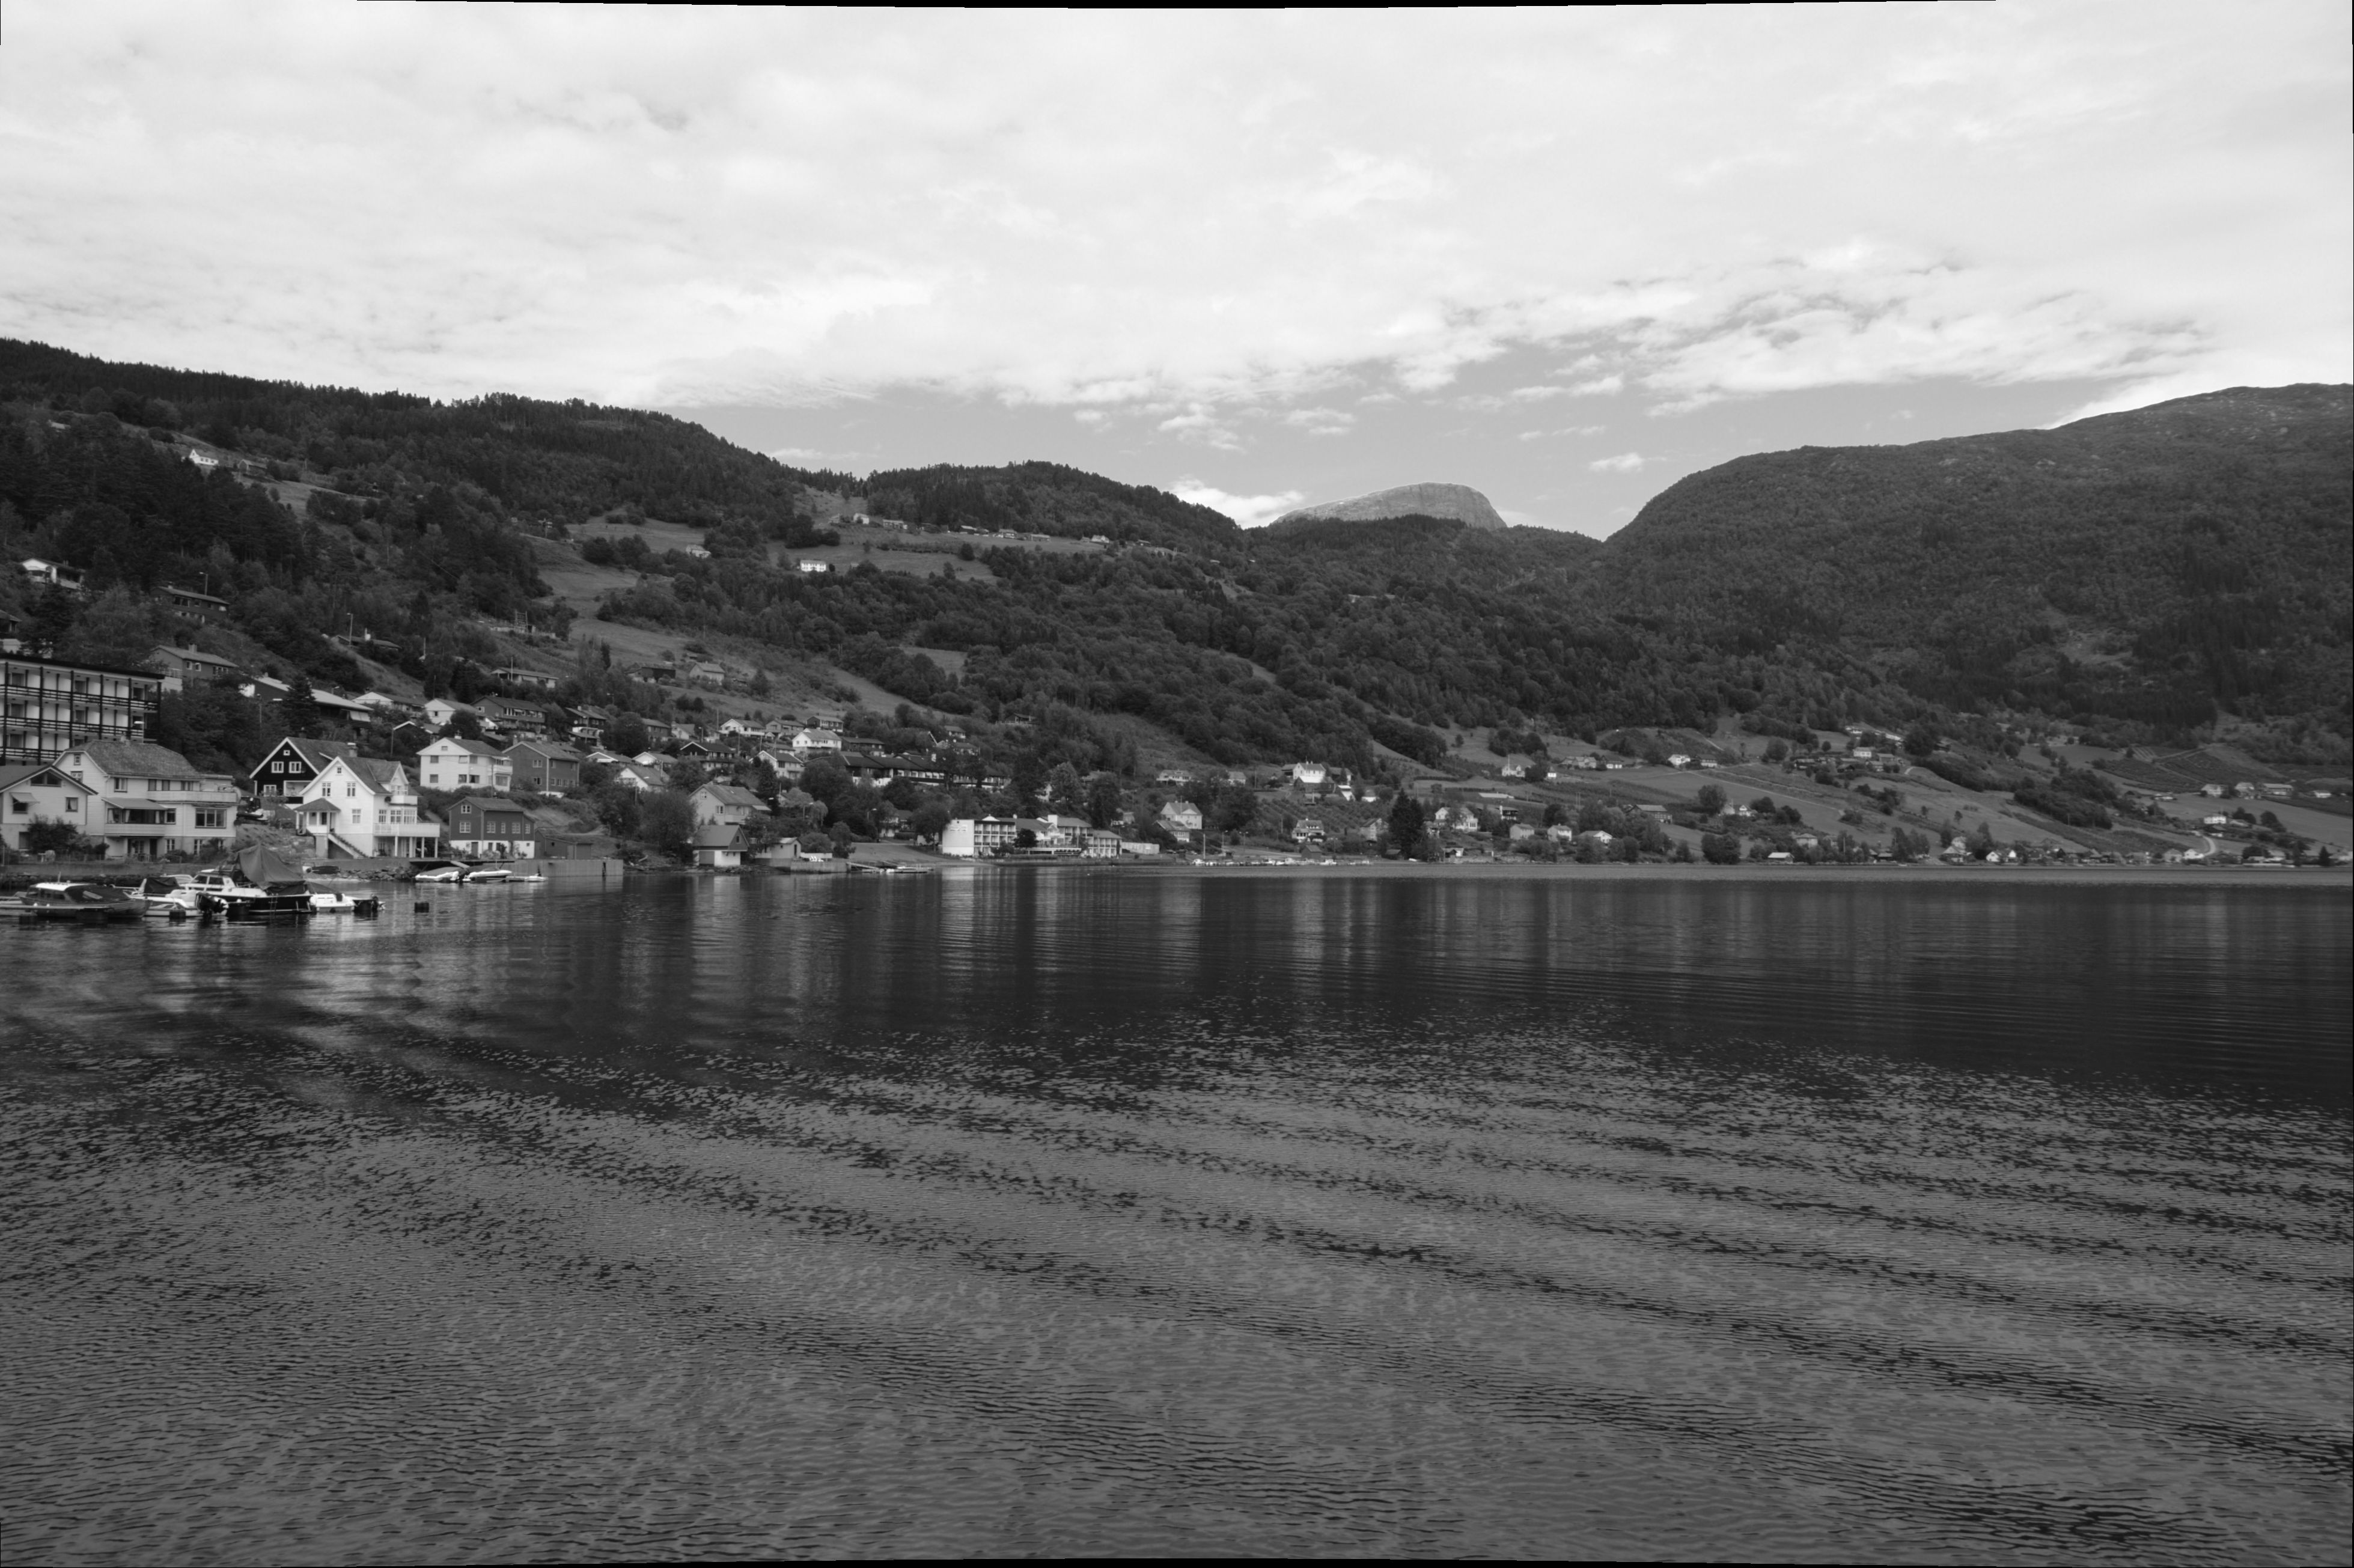
\includegraphics[width=0.5\linewidth]{bossbase_image00031.jpg}
		\caption{Grayscale PGM version of one of the RAW BOSSbase images. The lens frame can be seen on the image edges, particularly on the top edge.}
		\label{bossbase-image-with-frame-lens}
	\end{center}
\end{figure}


\subsection{Cropping} \label{sec:cropping}
This project studies the relationship between the number of bits embedded in an image and the total number of pixels in an image, in terms of a linear classifier's accuracy in detecting whether or not images have hidden payloads. Thus, I had to produce images of several different sizes -- the ultimate goal being to produce a graph with the total number of pixels on the x-axis and the classifier's accuracy on the y-axis.

I did this by taking ``central crops" of the images in each image set\footnote{Once again, I used \texttt{jpegtran} for this.}. A central crop retains the pixels in the middle of an image and crops pixels evenly from the top/bottom and left/right edges. I decided to use central crops -- rather than random crops, for instance -- since the main subject of an image is usually in, or near, the center. This meant that cropping preserved the general properties of the image sources and made for a more meaningful comparison of the classifier's performance on the large images relative to the small, cropped images. For example, if Actor3 takes pictures of people on the beach and I always crop towards the top-left corner, then the large images will have a lots of variations between neighbouring pixels because they capture the people whereas the smallest cropped versions will only capture the sky and be very smooth.

With my final graph in mind, I chose the dimensions I would crop my images to such that the total number of pixels in each image size would be linearly distributed on the x-axis.

As Actor3's images were my primary image set, I chose ten image sizes -- enough to make trends in the results easy to identify. I started with a smallest image size of $320\times240$, which was chosen to preserve the 4:3 ratio of the largest image size ($3072\times2304$). I computed the approximate difference in the number of pixels between consecutive image sizes ($\frac{1}{9} \cdot (3072 \cdot 2304 - 320 \cdot 240) \approx 777\,899$) and chose dimensions that produced approximately the right number of pixels while also preserving the 4:3 ratio. The resulting sizes are in Table \ref{actor3-sizes}.

\begin{table}[htbp]
    \begin{center}
        \begin{tabular}{ r  r | r}
        Width & Height & Total pixels \\ \hline
        320 & 240 & 76\,800 \\
        1\,056 & 792 & 836\,352 \\
        1\,472 & 1\,104 & 1\,625\,088 \\
        1\,792 & 1\,344 & 2\,408\,448 \\
        2\,048 & 1\,536 & 3\,145\,728 \\
        2\,304 & 1\,728 & 3\,981\,312 \\
        2\,528 & 1\,896 & 4\,793\,088 \\
        2\,720 & 2\,040 & 5\,548\,800 \\
        2\,912 & 2\,184 & 6\,359\,808 \\
        3\,072 & 2\,304 & 7\,077\,888 \\
        \end{tabular}
        \caption{Image sizes used for the Actor3 image set.}
        \label{actor3-sizes}
    \end{center}
\end{table}

I followed the same steps for BOSSbase, except I chose only eight image sizes and used $672\times896$ as the smallest size. Since it was my secondary image set, I wanted the images to be slightly smaller images and to have fewer image sizes to handle in order to speed up the experiments. Table \ref{bossbase-sizes} shows the resulting image sizes.

\begin{table}[htbp]
    \begin{center}
        \begin{tabular}{ r  r | r}
        Width & Height & Total pixels \\ \hline
        896 & 672 & 602\,112 \\
        1\,280 & 960 & 1\,228\,800 \\
        1\,536 & 1\,152 & 1\,769\,472 \\
        1\,792 & 1\,344 & 2\,408\,448 \\
        2\,016 & 1\,512 & 3\,048\,192 \\
        2\,172 & 1\,632 & 3\,544\,704 \\
        2\,368 & 1\,776 & 4\,205\,568 \\
        2\,560 & 1\,920 & 4\,915\,200 \\
        \end{tabular}
        \caption{Image sizes used for the BOSSbase image set.}
        \label{bossbase-sizes}
    \end{center}
\end{table}


\section{Embedding} \label{sec:juniward-impl}

A C++ implementation of J-UNIWARD available online \cite{binghamton-embedding} formed the basis of the implementation I used in my experiments, subject to a few important modifications.

An important property of this implementation is that the payload size must be specified in terms of bits per non-zero DCT coefficient. However, we are interested in specifying the payload as a specific number of bits -- this ensures that the same amount of information is embedded in each cover image, regardless of the coefficients. This preference has practical implications: users of an embedding algorithm will most generally be interested in the (approximate) detectability of a specific payload (like ``Meet me at 2pm") in an image of a particular size, without worrying about the number of non-zero coefficients. Thus, a feature I added was the ability to specify the payload size in bits.

Another important observation is that the implementation simulates ternary embedding whereas we are interested in binary embedding because it was used in \cite{2008-paper}\footnote{The differences between binary and ternary embedding were discussed in Section \ref{sec:distortion-function-min}}. Modifying J-UNIWARD to simulate binary instead of ternary embedding was a non-trivial change that involved updating the Payload-Limited Sender (PLS) implementation \cite{non-binary-embedding}. In general, however, ternary embedding is better because it can embed the same payload by making fewer changes and therefore achieve a lower detectability \cite{non-binary-embedding}.


\section{Costs} \label{sec:costs}

J-UNIWARD simulates embedding by computing a cost $c_i$ for changing each coefficient $x_i$ and then using these costs to compute the probability $\pi_i$ of changing $x_i$, according to the payload-limited sender formulation described in Section \ref{sec:distortion-function-min}.

In the original ternary implementation (i.e. the version prior to the modifications described in Section \ref{sec:juniward-impl}), there were costs for changing coefficient $x_i$ by $+1$ or $-1$ or not changing it at all (call them $c_i^{+1}$, $c_i^{-1}$, $c_i^{\ast}$, respectively). A characteristic of the resulting costs is $c_i^{+1} = c_i^{-1}$. However, since I use binary embedding, I only need the cost of making \textit{any} change -- whether it is $+1$ or $-1$ does not matter -- which is simply $c_i^{+1}$ (or equivalently $c_i^{-1}$).

By default, the J-UNIWARD implementation computes costs from scratch for each image. This is very inefficient since I need to simulate the embedding of many different payload lengths. A much better approach is to let J-UNIWARD compute and save the costs for each image once and read them whenever that image is used for embedding. My supervisor noticed this inefficiency prior to my project and had on hand a ``hacked" version of J-UNIWARD that saves the computed costs to a file and skips the embedding. He provided me with a copy of this code, which I used to compute the costs of all my images. I will refer to this version as J-UNIWARD-COSTS. Consequently, I had to modify the J-UNIWARD code once more to make it skip the cost computation and instead read the costs from a specified file.


\section{Features} \label{sec:features-impl}

I used a freely available \cite{binghamton-features} MATLAB implementation of the Cartesian-calibrated JPEG Rich Model (CC-JRM) out-of-the-box to generate image features. I did, however, have to write a script to convert the features (stored in one ASCII file per image) to a MATLAB matrix (stored as a \texttt{.MAT} file) with the fields expected by the classifier, which is discussed in Section \ref{sec:classifier-impl}.

A consequence of the design of JRM is that the sum of all features of an image is a constant. Thus, summing the features of my images was a sanity check that I ran occasionally.


\section{Classifier} \label{sec:classifier-impl}

As mentioned in \ref{sec:classifier-background}, I used a low-complexity linear classifier. A MATLAB implementation is available online \cite{binghamton-classifier} and I wrote a MATLAB script, based on the tutorial code that came with the implementation, to read the cover and stego image features from two \texttt{.MAT} files and run the classifier.


\section{Pipeline} \label{sec:pipeline}

Figure \ref{fig:experimental-design-flowchart} shows how all the components described in the previous sections come together.

\begin{figure}[htbp]
	\begin{center}
		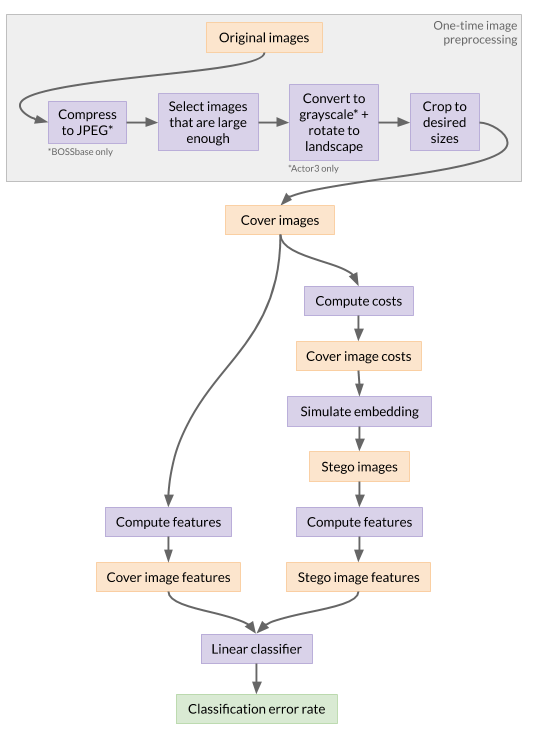
\includegraphics[width=\linewidth]{experimental_design_diagram.png}
		\caption{Experimental design flowchart.}
		\label{fig:experimental-design-flowchart}
	\end{center}
\end{figure}

The first step in the pipeline is the image preprocessing and cropping. This is done once per image set, producing eight (BOSSbase) or ten (Actor3) copies of the images -- one for each of the desired sizes. Then, each set of images of each size flows through the rest of the pipeline, independently of the others, once for each payload size.

To understand the rest of the pipeline, consider a concrete example: the $320\times240$ Actor3 images and a $12\,345$-bit payload. We need to feed the linear classifier the features of all $320\times240$ cover images and the features of their corresponding stego images, which we can compute in parallel.

The cover image features are simple: simply run JRM. For the stego images, we need to run J-UNIWARD-COSTS to compute the costs of changing the coefficients, run J-UNIWARD to simulate the embedding of a $12\,34$-bit payload in all the cover images, and finally run JRM to compute the features of the resulting stego images.


\section{Payload Sizes} \label{sec:payload-sizes}

Now that we have set up a clear path from cover images to classifier accuracy results, we can begin the experiments themselves. We are interested in studying the relationship between image size, in terms of pixels\footnote{Non-zero coefficients?}, and classifier accuracy using payloads of different sizes. In particular, our aim is to validate the square root law of steganography, a decade after it was first studied and tested \cite{2008-paper}. To mirror the results from the 2008 paper, we will run experiments with the following payload sizes (where $N$ is the number of pixels in an image):
\begin{itemize}
    \item Constant
    \item $\sim \sqrt{N}$
    \item $\sim \log{N}\cdot\sqrt{N}$
    \item $\sim N$
\end{itemize}

The first step in determining the concrete payload sizes is finding an image size/payload size pair that produced a reasonable probability of error. I aimed for around 20\%. After some educated trial-and-error (using the ternary J-UNIWARD implementation for Actor3 and my binary J-UNIWARD version for BOSSbase), I found the following:
\begin{itemize}
    \item Actor3: 0.3 bits per non-zero coefficient in $1056\times792$ pixel images had a minimal probability of error of 0.2249
    \item BOSSbase: $41\,287$ bits of payload (around 0.02 bits per pixel) in $1792\times1344$ pixel images had a minimal probability of error of 0.2028
\end{itemize}

For Actor3, I converted 0.3 bits per non-zero coefficient to the actual number of bits ($\sim 36\,223$) using the result of running a command line utility\footnote{I wrote this. It's called \texttt{JPEG-UTILS}. I will make this footnote better later.} that outputs the average number of non-zero coefficients.

For each image set, I chose a ``middle" image size such that the point on the graph for that size would have a error rate of around 20\%. I chose $2048\times1536$ for Actor3 and $1792\times1344$ for BOSSbase. Then, I needed to estimate the payload size needed to produce such an error rate in images of these two sizes.

Since $1792\times1344$ is the middle BOSSbase image size, no further calculations were necessary -- $41\,287$ is the desired number of bits.

For Actor3, on the other hand, an additional calculation was necessary. I computed following, under the assumption that the square root law holds:
\begin{equation}
    0.3 \cdot 120\,746 \cdot \sqrt{\frac{2048\cdot1536}{1056\cdot792}} \approx 70\,252
\end{equation}

In other words, if $70\,252$ bits are embedded in a $2048\times1536$ pixel Actor3 image, then we can expect the linear classifier to have an error rate of around 20\% given these stego images along with their corresponding cover images as input -- \textit{assuming the square root law holds}.

What we need next are four proportionality constants. As an example, let $r_2$ be the proportionality constant for the case where we embed a number of bits proportional to the square root of the number of pixels in an image. For each $W \times H$ image size, we will embed $r_2 \cdot \sqrt{N}$ bits of payload, where $N = W \cdot H$ is the number of pixels in the images. For each image set, we will compute the following four proportionality constants (where $N$ is the number of pixels in an image):
\begin{itemize}
    \item $r_1$: constant payload
    \item $r_2$: payload proportional to $\sqrt{N}$
    \item $r_3$: payload proportional to $\log{N} \cdot \sqrt{N}$
    \item $r_4$: payload proportional to $N$
\end{itemize}

Let $N_{mid}$ be the number of bits in the middle image size and let $m_{mid}^{\ast}$ be the number of bits that should be embedded in the middle image size to produce an error rate of around 20\%. For simplicity, we choose proportionality constants such that the same number of bits is embedded in the middle image in all four cases (i.e. when the payload is constant, $\sim \sqrt{N}$, $\sim \log{N} \cdot \sqrt{N}$, and $\sim N$).

Thus, we need to solve the following equations for $r_1,...,r_4$, knowing $N_{mid}$ and $m_{mid}^{\ast}$:
    \begin{align*}
    m^{\ast}_{mid} &= r_1 \\
    m^{\ast}_{mid} &= r_2 \cdot \sqrt{N_{mid}} \\
    m^{\ast}_{mid} &= r_3 \cdot \sqrt{N_{mid}} \cdot \log N_{mid} \\
    m^{\ast}_{mid} &= r_4 \cdot N_{mid}
    \end{align*}

For Actor3, $N_{mid} = 2048\cdot1536$ and $m_{mid}^{\ast}=70\,252$ and for BOSSbase, $N_{mid} = 1792 \cdot 2344$ and $m_{mid}^{\ast}=41\,287$. Thus, we get the following constants:

\begin{table}[htbp]
    \begin{center}
        \begin{tabular}{ r | r  r}
        & Actor3 & BOSSbase \\ \hline
        $r_1$ & 70252 & 41287 \\
        $r_2$ & 39.610 & 26.604 \\
        $r_3$ & 1.8351 & 1.2549 \\
        $r_4$ & 0.022333 & 0.017143 \\
        \end{tabular}
        \caption{Proportionality constants chosen for Actor3 and BOSSbase.}
        \label{fig:prop-constants}
    \end{center}
\end{table}

Finally we multiply these constants by 1, $\sqrt{N}$, $\log{N} \cdot \sqrt{N}$, and $N$ for each image size $W \times H$, where $N = W \cdot H$. The results of these calculations are in Appendix \ref{appendix:payload-sizes}.

In order to more closely mirror the results from \cite{2008-paper} (as well as provide more confident validation of the square root law), I computed two additional sets of proportionality constants. They were simply 30\% smaller and larger, respectively, than the constants above. These constants along with the resulting payload sizes are also found in Appendix \ref{appendix:prop-constants}.


\section{Experiments}

Now, everything is in place to run the experiments. This means running through the one-time preprocessing steps highlighted in Figure \ref{fig:experimental-design-flowchart} for each image set (i.e. once for Actor3 and once for BOSSbase) and then executing the rest of the pipeline once for each image size and payload size. Finally, I plotted all the results (namely the classifier's error rate for each image size/payload size pair), which is described in more detail in Chapter \ref{chap:results}.


%-----------------------
% split by question I'm answering, broken down by dataset
% emphasize/bold the conclusion within each section

\chapter{Results \& Analysis} \label{chap:results}

This chapter presents the experiment results and discusses how they align with our expectations. Overall, the experiments required \textbf{XXX} years of computing time and generated \textbf{XXX} TB of data in the form of images, features, and costs.

As we will see, Actor3 and BOSSbase produce similar results. Since Actor3 is the primary\footnote{Note to self: make sure I mention this early on - Experimental Design?} image set, most of the explanations and analysis of the results is in Section \ref{sec:actor3-results}. When I present the outcome of the BOSSbase experiments in Section \ref{sec:bossbase-results}, I will focus more on how the differences between the two image sets are reflected in the results.


\section{Experiment Result Visualizations}

Before presenting any results, I will explain the two visualization methods I chose.


\subsection{ROC Curves} \label{sec:roc-curves}

First, I will show \textbf{receiver operating characteristic (ROC) curves}. ROC curves plot the true positive rate (TPR), on the y-axis, against the false positive rate (FPR), on the x-axis, and are a standard tool for evaluating the diagnostic ability of a binary classifier. The TPR is equal to $1-f_n$ (where $f_n$ is the false negative rate) and is also called the \textbf{probability of detection}, while the FPR is written $f_r$ and is also called the \textbf{probability of false alarm}.

The points in an ROC curve can be used to compute the \textbf{minimum probability of error ($\bm{P_E}$)}: $P_E = \min{\frac{1}{2}(f_n+f_p)}$ over all points $(f_n, 1-f_p)$. Figure \ref{fig:actor3-roc-example} shows an example of an ROC curve with the minimum $P_E$ (referred to from now on as \textbf{MinPE}) point highlighted.

\begin{figure}[htbp]
	\begin{center}
		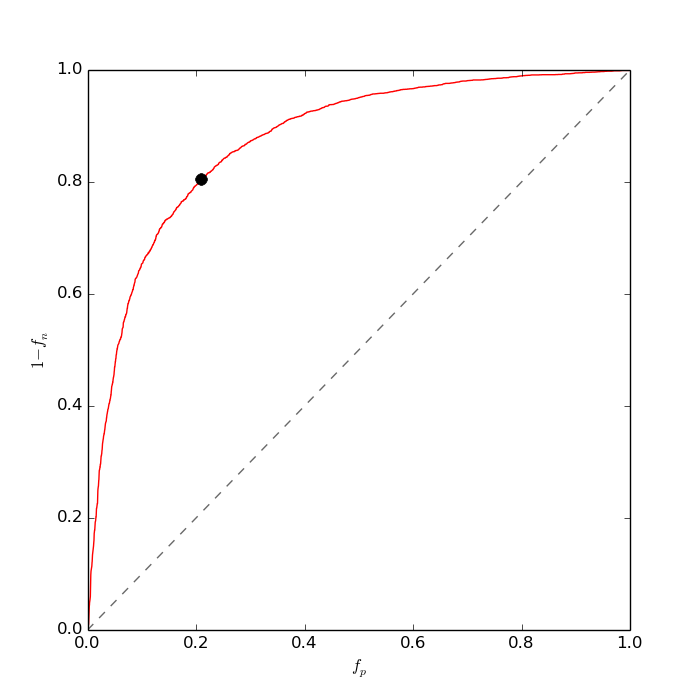
\includegraphics[width=0.5\linewidth]{actor3_size2048_70252b_roc.png}
		\caption{Actor3 example ROC curve. $2048\times1536$ images, $70\,252$ bits of payload in stego images. MinPE point highlighted. \textit{I will properly write this caption later.}}
		\label{fig:actor3-roc-example}
	\end{center}
\end{figure}

A straight line from the bottom-left corner to the top-right corner corresponds to the performance of a random classifier. On the other hand, the closer a curve is to the top-left corner, the closer the classifier is to perfection. Thus, if we identify the MinPE point on an ROC curve, we expect it to be one of the closest points to the top-left corner of the graph. The MinPE point is highlighted in Figure \ref{fig:actor3-roc-example}. Intuitively this makes sense because the top-left corner corresponds to $f_p = 0$ (no cover images are identified as stego images, in our case) and $1-f_n = 0 \implies f_n = 1$ (all stego images are identified as stego images).


\subsection{Detectability Versus Cover Size}

Second, I will plot detectability against cover size for each of the four payload rates (I will called these \textbf{detectability graphs}). But first, how should detectability be measured? \cite{2008-paper} considered three metrics (one being 1- MinPE) and they all exhibited similar results. Here we will only consider 1 - MinPE, which can be informally interpreted as the classifier's accuracy\footnote{Can it?}.

These graphs intentionally have a similar format to those in Section \ref{sec:2008-results} for ease of comparison. However, there are a couple of differences worth noting:
\begin{itemize}
	\item I express cover size as the number of pixels\footnote{As explained in Section \ref{sec:jpeg-compression}, JPEG compression produces an $8\times8$ block of coefficients for each $8\times8$ block of pixels, which means that the number of coefficients in a JPEG is equal to the number of pixels in the original raw image. Thus, I could equivalently express cover size as the number of (AC) DCT coefficients.}, whereas \cite{2008-paper} expresses cover size as the number of \textit{non-zero} (AC) DCT coefficients. Both units are correct in their respective contexts because they represent the number of places where embedding changes can be made: the nsF5 embedding algorithm used in \cite{2008-paper} ignores zero-valued coefficients, while J-UNIWARD uses all of them.
	\item I run experiments with four payload rates whereas \cite{2008-paper} only studies three payload rates. As I mentioned in Section \ref{sec:goals}, this is because the fourth rate ($\propto \sqrt{N} \cdot \log{N}$ where $N$ is the number of pixels) is only mentioned in \cite{2008-paper}'s conclusion as a potentially better measure of steganographic capacity for modern embedding algorithms that use adaptive embedding.
\end{itemize}


\section{Results From A Decade Ago} \label{sec:2008-results}

We first remind ourselves of what we hope our results will look like. Figure \ref{fig:2008-jpeg-results} shows the 2008 results from \cite{2008-paper} for the detection accuracy of a support vector machine-based classifier for nsF5 embedding in JPEG images.

There are three graphs: one for payloads that are constant (left), one for payloads proportional to the square root of the number of non-zero coefficients (middle), and one for payloads proportional to the number of non-zero coefficients (right). Each graph has three lines, corresponding to the use of three proportionality constants.

\begin{figure}[htbp]
	\begin{center}
		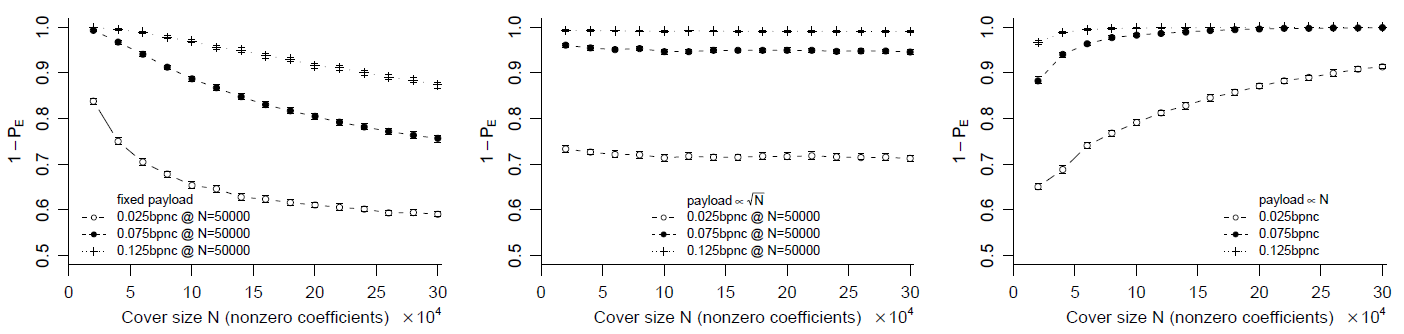
\includegraphics[width=\linewidth]{2008_jpeg_results.png}
		\caption{JPEG-domain results from \cite{2008-paper}}
		\label{fig:2008-jpeg-results}
	\end{center}
\end{figure}


\section{Actor3} \label{sec:actor3-results}

\subsection{ROC Curves} \label{sec:actor3-roc-curves}

Figure \ref{fig:actor3-roc-curves} presents ROC curves for each payload rate, using the payload sizes generated by the middle\footnote{By this I mean proportionality constants $r_1,...,r_4$ as opposed to those constants multiplied by $0.7$ or $1.3$, as described in Section \ref{sec:payload-sizes}.} proportionality constants. As explained in Section \ref{sec:roc-curves}, we can assess how well the classifier performs by how close a curve is to the top-left corner of the graph.

\begin{figure}[htbp]
    \centering
    \subfigure[Constant payload]{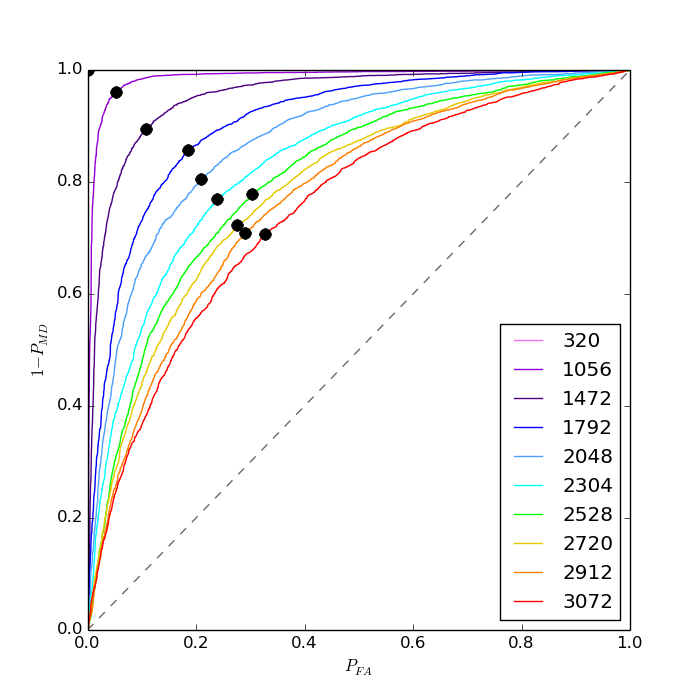
\includegraphics[width=0.45\linewidth]{actor3_roc_constant.png} \label{fig:actor3-roc-constant}}
    \subfigure[Payload $\propto \sqrt{N}$]{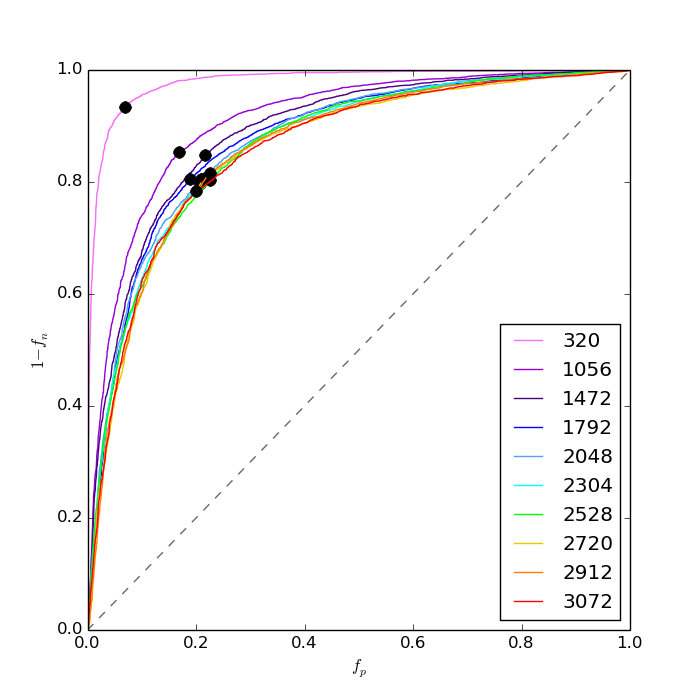
\includegraphics[width=0.45\linewidth]{actor3_roc_sqrt.png} \label{fig:actor3-roc-sqrt}}
    \subfigure[Payload $\propto \sqrt{N} \cdot \log{N}$]{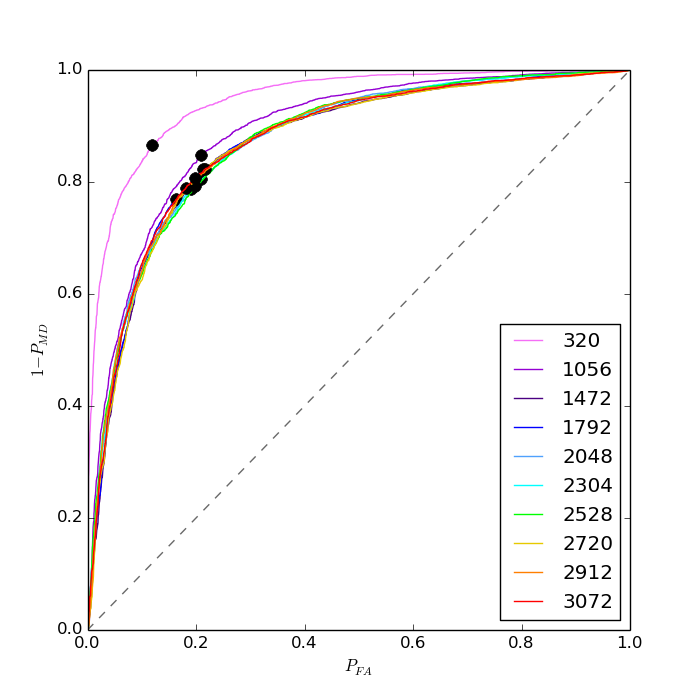
\includegraphics[width=0.45\linewidth]{actor3_roc_sqrt_log.png} \label{fig:actor3-roc-sqrt-log}}
    \subfigure[Payload $\propto N$]{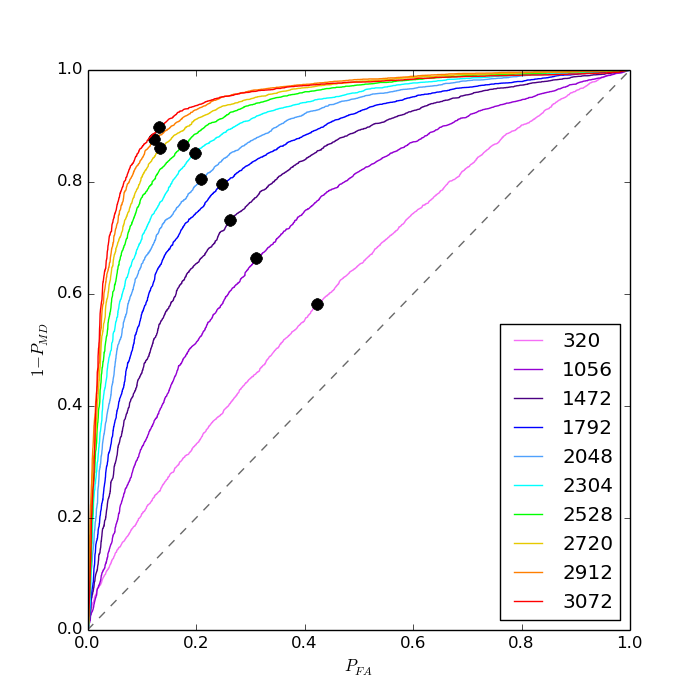
\includegraphics[width=0.45\linewidth]{actor3_roc_linear.png} \label{fig:actor3-roc-linear}}
    \caption{Actor3 ROC curves.}
    \label{fig:actor3-roc-curves}
\end{figure}

\paragraph{Constant payload} The classifier achieves perfect detection with the smallest image size -- its MinPE has coordinates $(0,1)$ which is why we can barely see it in Figure \ref{fig:actor3-roc-constant}. As image size increases, detector accuracy decreases and approaches that of a random classifier. This is to be expected since the number of potential embedding locations (coefficients) to choose from increases with cover size, so the distortion function is likely to be smaller\footnote{I'm not sure if this is clear.}.

\paragraph{Payload $\bm{\propto \sqrt{N}}$ and $\bm{\propto \sqrt{N} \cdot \log{N}}$} The curves and MinPE points are very close together in both Figures \ref{fig:actor3-roc-sqrt} and \ref{fig:actor3-roc-sqrt-log}, with the notable exception of the curves for the smallest image size. These two curves correspond to $10\,976$ and $8\,253$ bits of payload, respectively, which is a very high proportion (10-15\%) of the number of pixels in the cover images. The effect of embedding such a large payload trumps the fact that the payload is proportional to some function of the number of pixels in each cover image\footnote{Is there a better/more formal way of expressing this?}. Thus, we can safely ignore these two curves. The rest of the curves, however, show that detectability is approximately constant for both payload rates. The curves in Figure \ref{fig:actor3-roc-sqrt-log} are visibly closer together than those in Figure \ref{fig:actor3-roc-sqrt}, suggesting that steganographic capacity (using modern embedding algorithms\footnote{\textit{I will elaborate more...}}) is more accurately measured as being of order $\sqrt{N} \cdot \log{N}$ than of order $\sqrt{N}$, where $N$ is the number of cover image pixels.

\paragraph{Payload $\bm{\propto N}$} The first thing we observe is that Figure \ref{fig:actor3-roc-linear} shows the exact opposite of the trend in Figure \ref{fig:actor3-roc-constant}: as image size increases, detector accuracy \textit{increases}. This is easy to see by comparing the two graphs and observing that the order in which the curve colours appear in each graph is reversed. Given our empirical observations about how the square root law appears to hold in practice, this behaviour is not surprising: as image size (measured in terms of the number of pixels $N$) increases, $r_4N - r_2\sqrt{N}$ (for proportionality constants $r_2, r_4$) increases. This means that, for fixed proportionality constants, the linear payloads exceed the images' steganographic capacity by larger and larger margins, which is increasingly detectable. Another interesting observation is that the curves are all closer to the line depicting a random classifier's accuracy. This is not a result of the payload rate, but rather it is a result of the choice of proportionality constant choice -- if the constant was larger, the curves would have all been closer to the top-left corner. Figure \ref{fig:actor3-roc-linear-all-constants} shows the ROC curves for all three proportionality constants: $0.7 \cdot r_4, r_4, 1.3 \cdot r_4$.

\begin{figure}[htbp]
    \centering
    \subfigure[$0.7 r_4$]{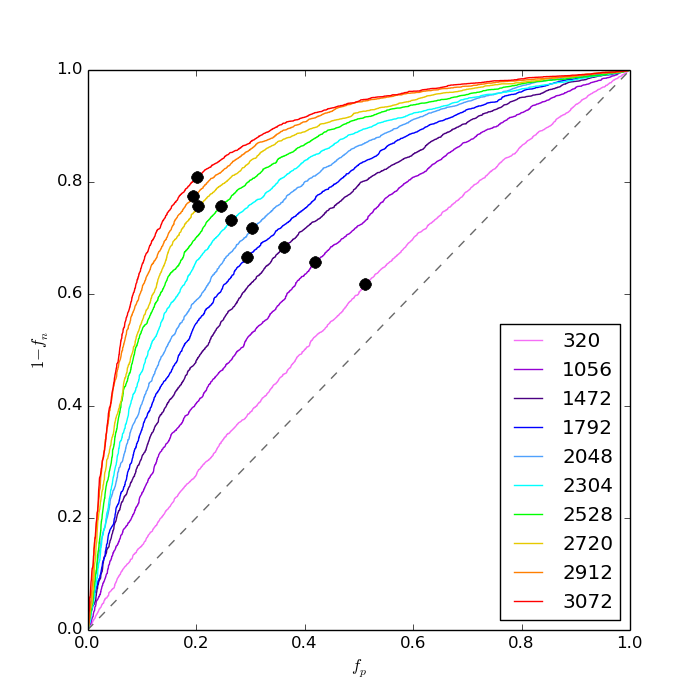
\includegraphics[width=0.3\linewidth]{actor3_roc_linear_small_constant.png}}
    \subfigure[$r_4$]{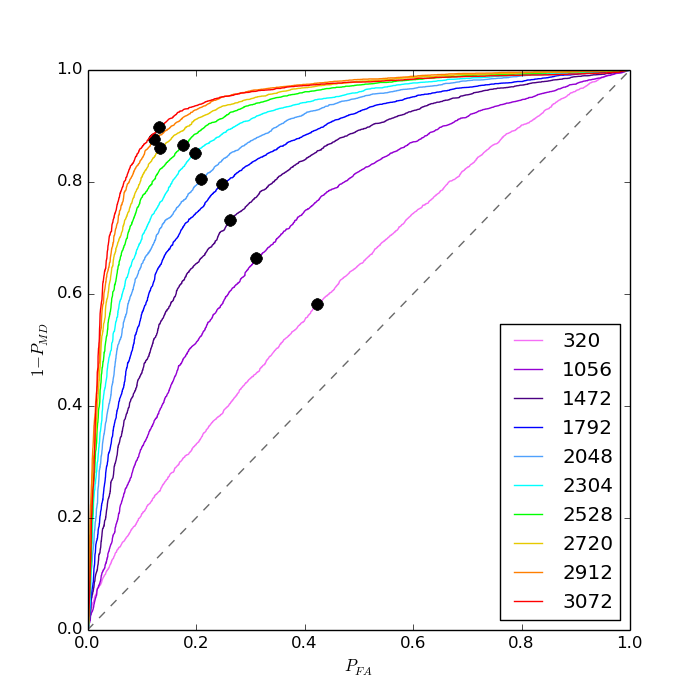
\includegraphics[width=0.3\linewidth]{actor3_roc_linear.png}}
    \subfigure[$1.3 r_4$]{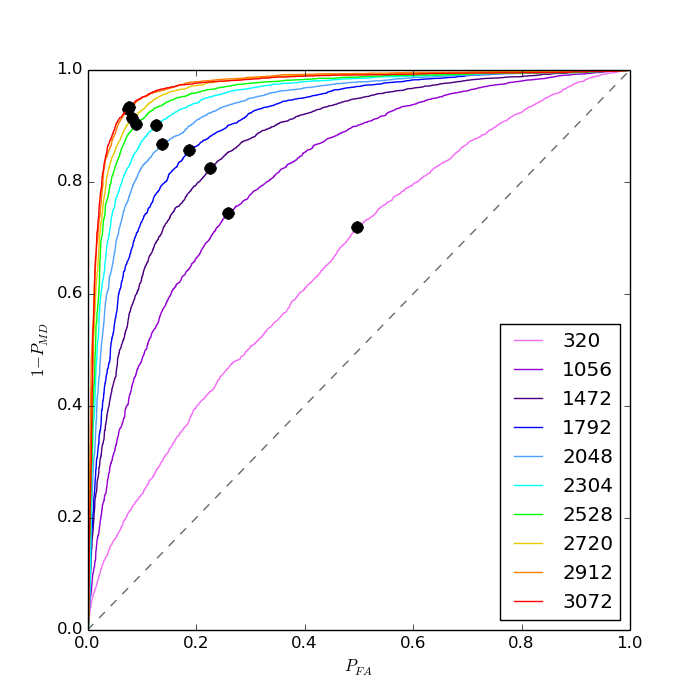
\includegraphics[width=0.3\linewidth]{actor3_roc_linear_large_constant.png}}
    \caption{Actor3 ROC curves for linear payloads. All constants.}
    \label{fig:actor3-roc-linear-all-constants}
\end{figure}


\subsection{Detectability Versus Cover Size} \label{sec:actor3-detectability-analysis}

In Figure \ref{fig:actor3-detectability-graphs} we see 1 - MinPE plotted against cover size, where the MinPE points are precisely those highlighted in Figure \ref{fig:actor3-roc-linear-all-constants}. It is more straightforward to assess changes in detectability with these graphs than with ROC curves because we can compare the detectability metric (MinPE) directly on the y-axis.

\begin{figure}[htbp]
    \centering
    \subfigure[Constant payload]{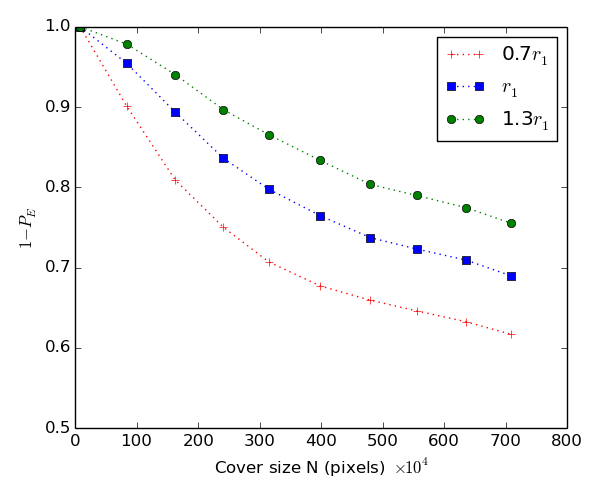
\includegraphics[width=0.45\linewidth]{actor3_detectability_constant.png} \label{fig:actor3-detectability-constant}}
    \subfigure[Payload $\propto \sqrt{N}$]{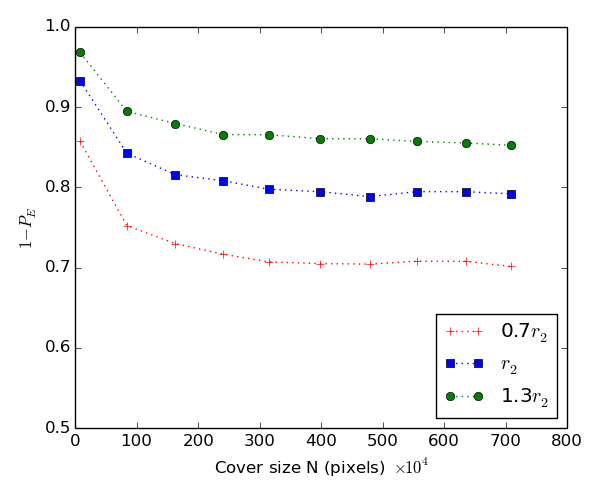
\includegraphics[width=0.45\linewidth]{actor3_detectability_sqrt.png} \label{fig:actor3-detectability-sqrt}}
    \subfigure[Payload $\propto \sqrt{N} \cdot \log{N}$]{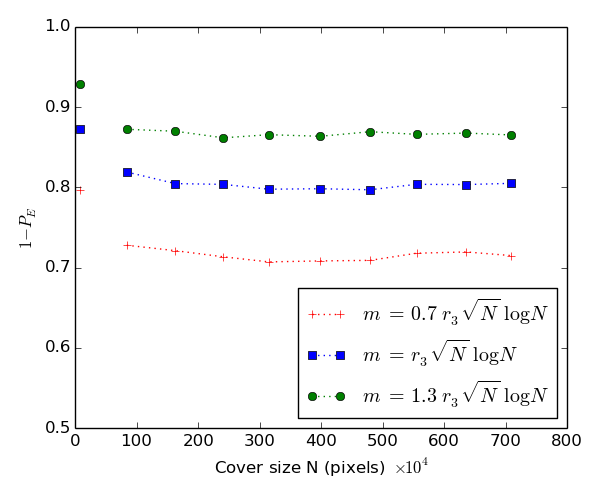
\includegraphics[width=0.45\linewidth]{actor3_detectability_sqrt_log.png} \label{fig:actor3-detectability-sqrt-log}}
    \subfigure[Payload $\propto N$]{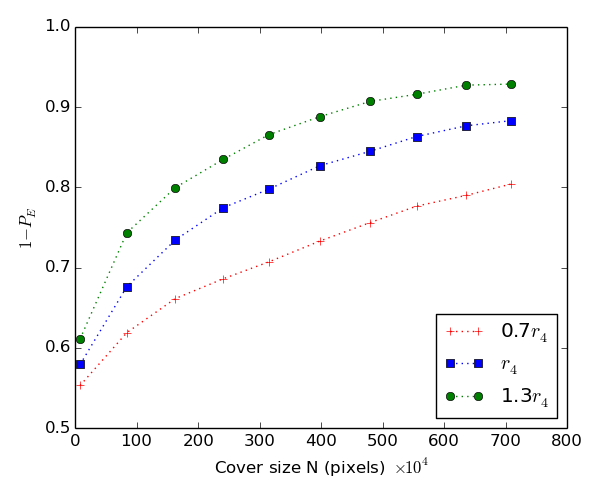
\includegraphics[width=0.45\linewidth]{actor3_detectability_linear.png} \label{fig:actor3-detectability-linear}}
    \caption{Actor3 detectability graphs.}
    \label{fig:actor3-detectability-graphs}
\end{figure}

The trends for each payload rate that were discussed in Section \ref{sec:actor3-roc-curves} are very clearly visible here:
\begin{itemize}
	\item Detectability decreases as image size increases for constant payloads, which we can see in Figure \ref{fig:actor3-detectability-constant}.
	\item Figures \ref{fig:actor3-detectability-sqrt} and \ref{fig:actor3-detectability-sqrt-log} show that detectability is approximately constant for payloads that are both $\propto \sqrt{N}$ and $\propto \sqrt{N} \cdot \log{N}$, respectively. The fact that the ROC curves were closer together for payloads $\propto \sqrt{N} \cdot \log{N}$ than for payloads $\propto \sqrt{N}$ manifests itself here as well: the lines in Figure \ref{fig:actor3-detectability-sqrt-log} are flatter than those in Figure \ref{fig:actor3-detectability-sqrt} (ignoring the points for the smallest image size, which we also disregarded when assessing the ROC curves).
	\item The concurrent increase in image size and detectability for payloads $\propto N$ can be seen in Figure \ref{fig:actor3-detectability-linear}
\end{itemize}


\section{BOSSbase} \label{sec:bossbase-results}

\subsection{ROC Curves} \label{sec:bossbase-roc-curves}

Figure \ref{fig:bossbase-roc-curves} shows the ROC curves for BOSSbase. There is an evident similarity between these curves and the curves for Actor3 in Figure \ref{fig:actor3-roc-curves} for all four payload rates.

Before discussing the similarities, we must first understand why the experiments were repeated on two different sets of images: it is \textit{not} the case that because the square root law appears to hold with the Actor3 images, it will necessarily hold for another image set, like BOSSbase. This is because with any set of images, there is a chance that the images have some properties in common that causes embedders and detectors to behave in a certain way. For instance, if a high proportion of user A's pictures are zoomed in on grains of sand whereas user B mostly takes pictures of the clear blue sky, detectability will almost certainly be higher in all of user B's images, regardless of the payload rate\footnote{This is an extreme example, but serves to illustrate the point that image sets can have properties that alter the behaviour of embedders and therefore detectors. This is not limited to the subject of the images, which is in fact one of the least important properties of a set of images in practice. An example of a more important property is the ISO setting (which specifies sensitivity to light) of the camera when the images are taken.}. This fact is particularly relevant for Actor3 because all the images were taken by the same user with the same camera (and likely the same camera settings). Hence, it is particularly important to validate our Actor3 experiment findings on another image set. BOSSbase is a good choice because it contains images taken with seven different cameras, so if we observe similar behaviour again then it is likely be a general trend rather than a trend specific to the image set.

With this in mind, we can be pleased to see that the BOSSbase images behaved in a similar way to the Actor3 images. If the ROC curves or detectability graphs had exposed \textit{different} behaviours, then the experiments would have had to be repeated a third time with yet another image set as a majority vote\footnote{Is this clear/accurate?}.

Therefore, all the analysis in Section \ref{sec:actor3-roc-curves} applies here as well, though with a few slight differences that are worth noting:
\begin{itemize}
	\item The smallest BOSSbase image size does not stand out as much as in Actor3, in the sense that the BOSSbase ROC curves in Figures \ref{fig:bossbase-roc-sqrt} and \ref{fig:bossbase-roc-sqrt-log} are very close to the ROC curves for the other image sizes. This is in contrast with the ROC curves for the smallest Actor3 image size in Figures \ref{fig:actor3-roc-sqrt} and \ref{fig:actor3-roc-sqrt-log}, which are noticeably different from the ROC curves of the other Actor3 image sizes. This difference is not surprising: the smallest BOSSbase images have around 10 times as many pixels as the Actor3 images but the number of payload bits as a proportion of the number of pixels is 14\% for Actor3's smallest images but only 3\% for BOSSbase's smallest images (when the payload is $\propto \sqrt{N}$, as an example). Thus, a much larger proportion of the pixels (coefficients, to be precise) need to be used for embedding in Actor3's smallest images, resulting in higher detectability. This could have been avoided by choosing the same image sizes for both image sets.
	\item The ROC curves for the constant payloads and payloads $\propto N$ are much more spread out for Actor3 in Figures \ref{fig:actor3-roc-constant} and \ref{fig:actor3-roc-linear} than for BOSSbase in Figures \ref{fig:bossbase-roc-constant} and \ref{fig:bossbase-roc-linear}. Once again, this can be attributed to the fact that different image sizes were chosen for the two image sets. Specifically, the difference in the number of pixels between consecutive image sizes is larger for Actor3 ($800\,000$ pixels) than for BOSSbase ($700\,000$ pixels), so consecutive image sizes can be expected to behave more similarly for BOSSbase than for Actor3.
\end{itemize}

\begin{figure}[htbp]
    \centering
    \subfigure[Constant payload]{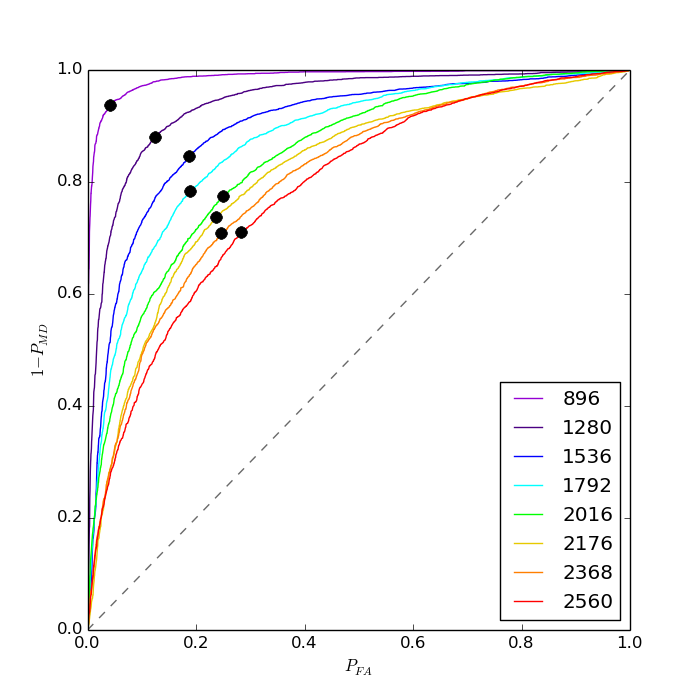
\includegraphics[width=0.45\linewidth]{bossbase_roc_constant.png} \label{fig:bossbase-roc-constant}}
    \subfigure[Payload $\propto \sqrt{N}$]{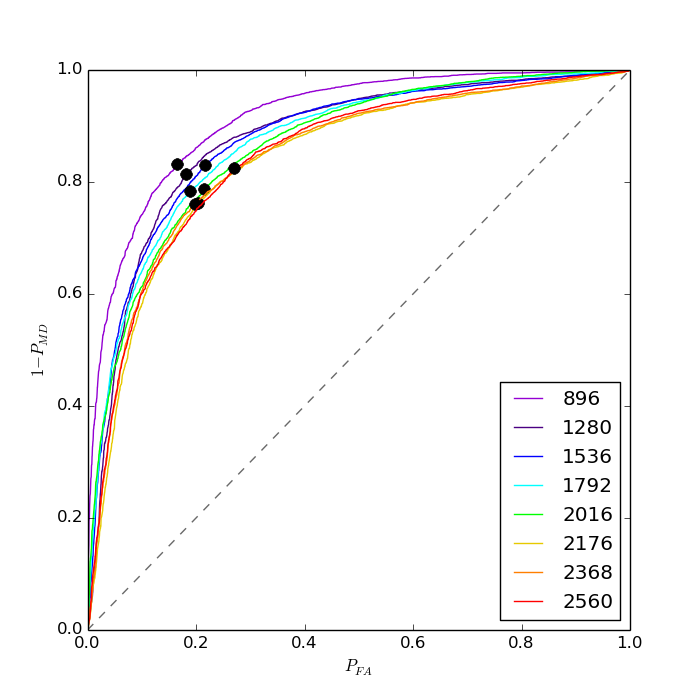
\includegraphics[width=0.45\linewidth]{bossbase_roc_sqrt.png} \label{fig:bossbase-roc-sqrt}}
    \subfigure[Payload $\propto \sqrt{N} \cdot \log{N}$]{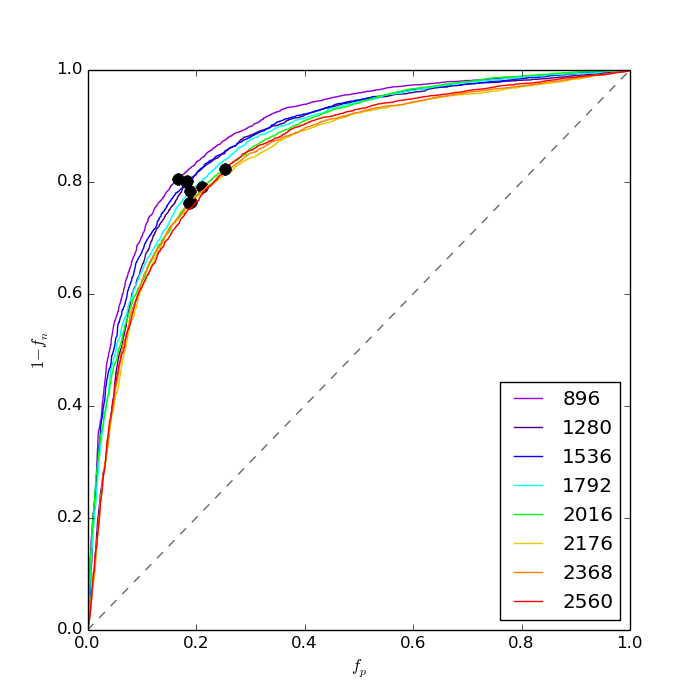
\includegraphics[width=0.45\linewidth]{bossbase_roc_sqrt_log.png} \label{fig:bossbase-roc-sqrt-log}}
    \subfigure[Payload $\propto N$]{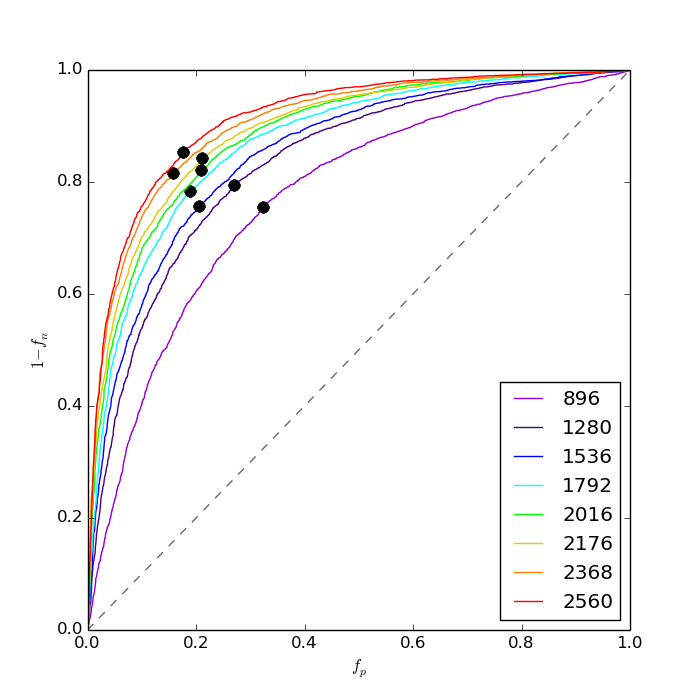
\includegraphics[width=0.45\linewidth]{bossbase_roc_linear.png} \label{fig:bossbase-roc-linear}}
    \caption{BOSSbase ROC curves.}
    \label{fig:bossbase-roc-curves}
\end{figure}


\subsection{Detectability Versus Cover Size}

Given the similarity of the BOSSbase and Actor3 ROC curves, the detectability graphs for BOSSbase are unsurprisingly similar to those for Actor3.

As noted in the ROC curve analysis in Section \ref{sec:bossbase-roc-curves}, the smallest BOSSbase image size does not stand out in Figures \ref{fig:bossbase-detectability-sqrt} and \ref{fig:bossbase-detectability-sqrt-log} as much as the smallest Actor3 image size does in Figures \ref{fig:actor3-detectability-sqrt} and \ref{fig:actor3-detectability-sqrt}.

Most notably, the square root law is more closely obeyed for payloads $\propto \sqrt{N} \cdot \log{N}$ than for payloads $\propto \sqrt{N}$, which is a bit more visible here than in Figure \ref{fig:actor3-detectability-graphs}. Otherwise, the Actor3 analysis in Section \ref{sec:actor3-detectability-analysis} also applies here.

\begin{figure}[htbp]
    \centering
    \subfigure[Constant payload]{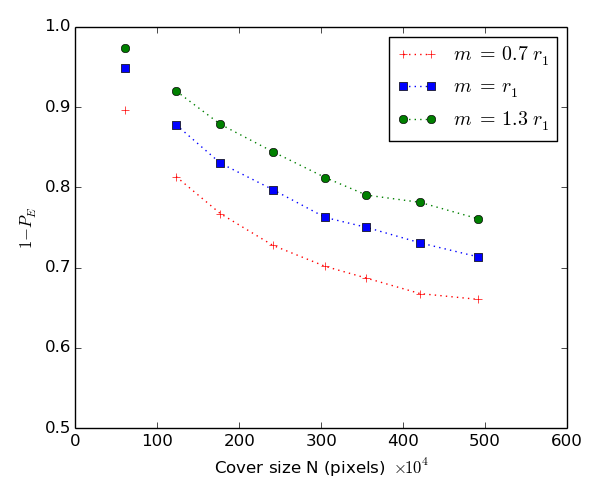
\includegraphics[width=0.45\linewidth]{bossbase_detectability_constant.png} \label{fig:bossbase-detectability-constant}}
    \subfigure[Payload $\propto \sqrt{N}$]{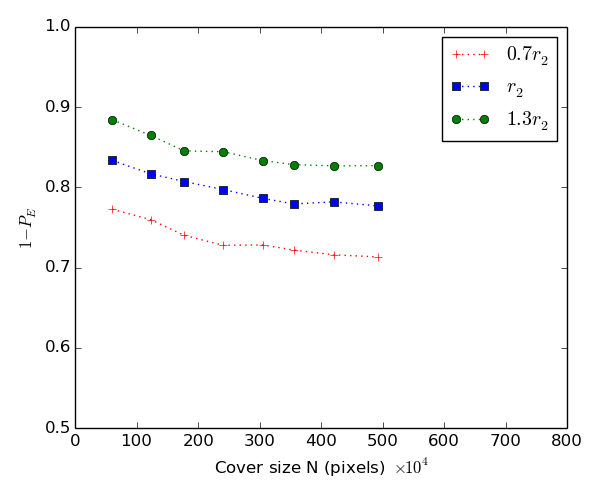
\includegraphics[width=0.45\linewidth]{bossbase_detectability_sqrt.png} \label{fig:bossbase-detectability-sqrt}}
    \subfigure[Payload $\propto \sqrt{N} \cdot \log{N}$]{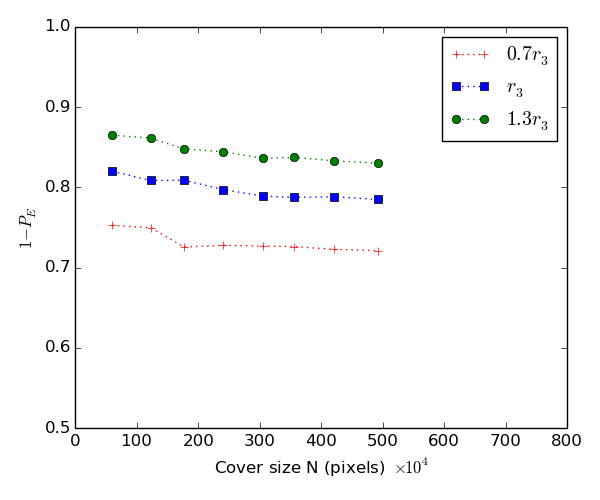
\includegraphics[width=0.45\linewidth]{bossbase_detectability_sqrt_log.png} \label{fig:bossbase-detectability-sqrt-log}}
    \subfigure[Payload $\propto N$]{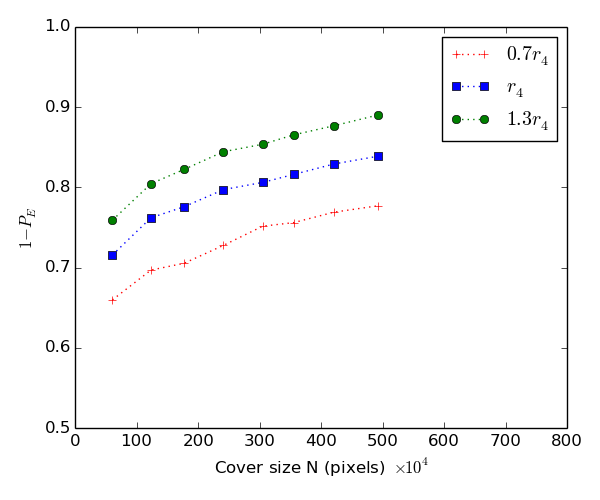
\includegraphics[width=0.45\linewidth]{bossbase_detectability_linear.png} \label{fig:bossbase-detectability-linear}}
    \caption{BOSSbase detectability graphs. X-axis max value is 800 to make it comparable with Actor3 results.}
    \label{fig:bossbase-detectability-graphs}
\end{figure}



%-----------------------
\chapter{Conclusion}

Perhaps the best summary of why the empirical validation of the square root law is significant is the following quote from \cite{laboratory-to-real-world}: \textit{``What is remarkable about the square root law is that, although both asymptotic and proved only for artificial sources, it is robust and manifests in real life''}.

The square root law was first shown to hold in practice in 2008 \cite{2008-paper} in both the spatial domain (raw images) and the JPEG domain using formerly state-of-the-art steganography and steganalysis techniques. We have shown that the law continues to hold in the DCT domain -- in fact, we observed that steganographic payload capacity is of order $\sqrt{N} \log{N}$ rather than $\sqrt{N}$ for images with $N$ pixels, which reflects the use current state-of-the-art adaptive embeddding algorithms.

Our experimental results on two large image sets align with the results from \cite{2008-paper} and confirm our hypothesis from Section \ref{sec:hypothesis}. They can be summarized as follows (where $N$ is the number of pixels in an image):
\begin{itemize}
	\item For constant payloads, detectability decreases as image size increases.
	\item For payloads $\propto \sqrt{N}$ or $\propto \sqrt{N} \cdot \log{N}$, detectability is approximately constant as image size increases.
	\item For payloads $\propto N$, detectability increases as image size increases.
\end{itemize}

\footnote{Do I need to reiterate/justify here that $\sqrt{N}\log{N}$ is better than $\sqrt{N}$?}


\section{Further Work}

Although this project provides much-needed fresh results regarding the manifestation of the square root law in the real world, there is always more work to be done. The embedding and detection tools that we tested are \textit{currently} the state-of-the-art, but will no longer hold this title in a few years as both steganography and steganalysis progress. Once a new suite of tools are developed, tested, and put to use, another empirical study will be in order.

In particular, there have already been breakthroughs in the use of deep learning for steganalysis. For instance, \cite{steganalysis-cnn} describes a convolutional neural network for JPEG steganalysis based on the modern use of features that are aware of the JPEG phase. The network is tested on two embedding algorithms (one of which is J-UNIWARD) and reveals promising results. Another recent example is the deep residual network architecture developed in \cite{deep-residual-network} that provides both spatial domain and JPEG domain steganalysis and performs significantly better than existing steganalysis techniques, particularly in the JPEG domain.

It would be very interesting to conduct further research into whether a square root law even \textit{exists} for deep learning-based steganalysis (and potentially steganography) and what form it takes. Research on applying deep learning to steganography continues to grow and develop and it is certainly possible that current state-of-the-art embedding and detection techniques will be rendered obsolete in just a few years.


%-----------------------
\bibliography{mybib}{}
\bibliographystyle{plain}


%-----------------------
\begin{appendices}

\chapter{} \label{appendix:payload-sizes}

\section{Proportionality Constants} \label{appendix:prop-constants}

\begin{table}[htbp]
    \begin{center}
        \begin{tabular}{ r | r  r}
        & Actor3 & BOSSbase \\ \hline
        $0.7 \cdot r_1$ & 49176 & 28900 \\
        $r_1$ & 70252 & 41287 \\
        $1.3 \cdot r_1$ & 91327 & 53673 \\ \hline
        $0.7 \cdot r_2$ & 27.727 & 18.623 \\
        $r_2$ & 39.610 & 26.604 \\
        $1.3 \cdot r_2$ & 51.492 & 34.585 \\ \hline
        $0.7 \cdot r_3$ & 1.2845 & 0.87844 \\
        $r_3$ & 1.8351 & 1.2549 \\
        $1.3 \cdot r_3$ & 2.3856 & 1.6314 \\ \hline
        $0.7 \cdot r_4$ & 0.015633 & 0.012000 \\
        $r_4$ & 0.022333 & 0.017143 \\
        $1.3 \cdot r_4$ & 0.029032 & 0.022285 \\
        \end{tabular}
        \caption{Proportionality constants chosen for Actor3 and BOSSbase.}
    \end{center}
\end{table}

To be added here:
\begin{itemize}
    \item All payload sizes
\end{itemize}

\end{appendices}

\end{document}